\section{Numerical examples}
\label{section: Chapter5/examples}

Finally, both the proposed E-P-D model and the E-P-PD model are applied to simulate a three-point bending experiment in \Cref{section: Chapter5/examples/3pb} and the experiment adopted for the Sandia Fracture Challenge in \Cref{section: Chapter5/examples/SFC}.

%%%%%%%%%%%%%%%%%%%%%%%%%%%%%%%%%%%%%%%%%%%%%%%%%%%%%%%%%%%%%%%%%%%%%%%%%%%%%%%%%%%%%%%%%%%
%%%%%%%%%%%%%%%%%%%%%%%%%%%%%%%%%%%%%%%%%%%%%%%%%%%%%%%%%%%%%%%%%%%%%%%%%%%%%%%%%%%%%%%%%%%
%%%%%%%%%%%%%%%%%%%%%%%%%%%%%%%%%%%%%%%%%%%%%%%%%%%%%%%%%%%%%%%%%%%%%%%%%%%%%%%%%%%%%%%%%%%
%%%%%%%%%%%%%%%%%%%%%%%%%%%%%%%%%%%%%%%%%%%%%%%%%%%%%%%%%%%%%%%%%%%%%%%%%%%%%%%%%%%%%%%%%%%
%%%%%%%%%%%%%%%%%%%%%%%%%%%%%%%%%%%%%%%%%%%%%%%%%%%%%%%%%%%%%%%%%%%%%%%%%%%%%%%%%%%%%%%%%%%
%%%%%%%%%%%%%%%%%%%%%%%%%%%%%%%%%%%%%%%%%%%%%%%%%%%%%%%%%%%%%%%%%%%%%%%%%%%%%%%%%%%%%%%%%%%
%%%%%%%%%%%%%%%%%%%%%%%%%%%%%%%%%%%%%%%%%%%%%%%%%%%%%%%%%%%%%%%%%%%%%%%%%%%%%%%%%%%%%%%%%%%
%%%%%%%%%%%%%%%%%%%%%%%%%%%%%%%%%%%%%%%%%%%%%%%%%%%%%%%%%%%%%%%%%%%%%%%%%%%%%%%%%%%%%%%%%%%
%%%%%%%%%%%%%%%%%%%%%%%%%%%%%%%%%%%%%%%%%%%%%%%%%%%%%%%%%%%%%%%%%%%%%%%%%%%%%%%%%%%%%%%%%%%
%%%%%%%%%%%%%%%%%%%%%%%%%%%%%%%%%%%%%%%%%%%%%%%%%%%%%%%%%%%%%%%%%%%%%%%%%%%%%%%%%%%%%%%%%%%
\subsection{Three-point bending}
\label{section: Chapter5/examples/3pb}

With modeling choices motivated and demonstrated in \Cref{section: Chapter5/verification/homogenized,section: Chapter5/verification/nonhomogeneous}, the model is now applied to simulate a three-point bending experiment for a specimen composed of an aluminum alloy \cite{kubik2019ductile}. In particular, we focus attention on the comparison of the E-P-PD model and the proposed E-P-D model with coalescence dissipation.

First, material properties and model parameters are calibrated against a tension test of a notched cylindrical specimen (R13 notch). Details of the specimen geometry, experimental setup and force-displacement data are provided in \cite{kubik2018notched}. Our calculations employ a cylindrical coordinate system, and symmetry is assumed about both the centerline and the half-plane of the specimen. The finite element mesh for this problem is shown in \Cref{fig: Chapter5/3pb/mesh}. \texttt{QUAD4} elements are used to discretize the domain with a structured mesh. The maximum and the minumum element sizes are \SI{1}{\milli\meter} and \SI{0.0625}{\milli\meter}, respectively.

\begin{figure}[!htb]
  \centering
  \tikzsetnextfilenamesafe{Chapter5/3pb/mesh}
  \begin{tikzpicture}
    \node[inner sep=0] (mesh) at (0,0) {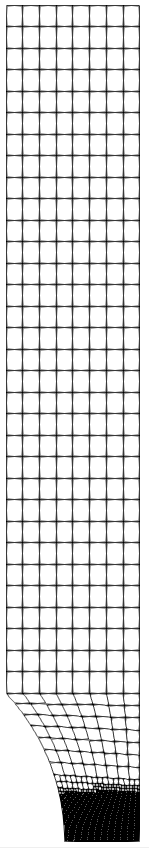
\includegraphics[width=0.09\textwidth,scale=0.5]{Chapter5/figures/3pb/mesh}};
    \node (box) at (mesh.south west) [draw,blue,thick,minimum width=0.09\textwidth,minimum height=51,anchor=south west] {};
    \node[inner sep=0] (meshzoom) at (7,0) {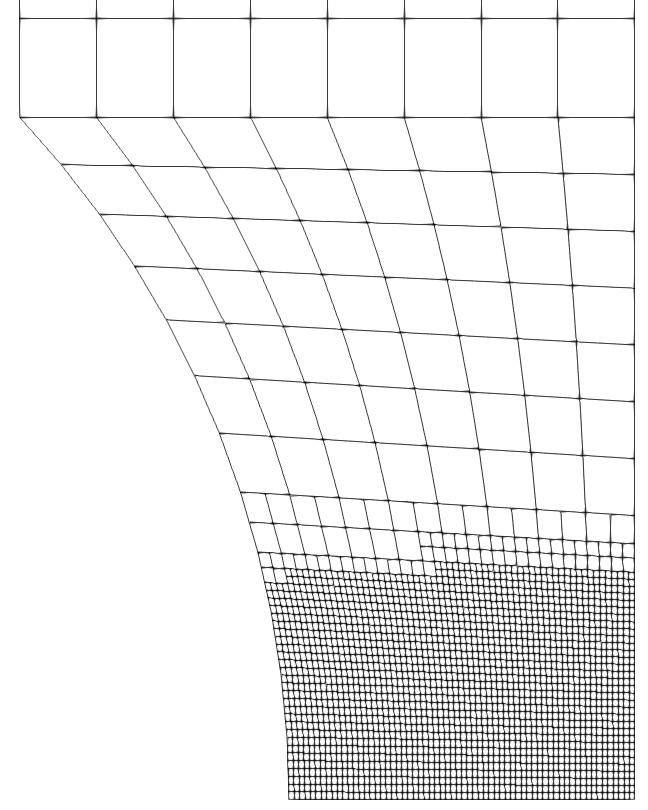
\includegraphics[width=0.36\textwidth,scale=0.5]{Chapter5/figures/3pb/mesh_zoom}};
    \node (boxzoom) at (meshzoom.south west) [draw,blue,thick,minimum width=0.36\textwidth,minimum height=210,anchor=south west] {};
    \draw (box.north east) -- (boxzoom.north west);
    \draw (box.south east) -- (boxzoom.south west);
  \end{tikzpicture}
  \caption{The mesh used for calibration and the zoomed-in view of the refined region.}
  \label{fig: Chapter5/3pb/mesh}
\end{figure}


Calibrated material properties and model parameters are summarized in \Cref{tab: Chapter5/3pb}. The E-P-D model is calibrated using a range of $\beta$ and $\varepsilon_0$ values. The corresponding force-displacement curves are shown in \Cref{fig: Chapter5/3pb/force_disp}.

We note that a significantly larger critical fracture energy $\psi_c$ is required for the E-P-PD model for the onset of damage to match the experiment. This is expected as the generalized fracture driving energy for the E-P-PD model includes contributions from plasticity, while only the active strain energy contributes to crack growth in the E-P-D model. According to \eqref{eq: upper bound}, polyconvexity requires a phase-field regularization length $l \leq \SI{0.01}{\milli\meter}$.

\begin{table}[htb!]
  \scriptsize
  \centering
  \caption{Summary of the calibrated material properties and model parameters}
  \begin{tabular}{r | c | c | c | c}
    \toprule
    Property/Parameter            & Symbol          & Value(E-P-D)                   & Value(E-P-PD)              & Unit                                       \\
    \midrule
    Young's modulus               & $E$             & \SI{7.25e4}{}                  & \SI{7.25e4}{}              & \SI{}{\mega\pascal}                        \\
    Poisson's ratio               & $\nu$           & 0.34                           & 0.34                       & nondim.                                    \\
    \midrule
    Yield stress                  & $\sigma_y$      & 345                            & 345                        & \SI{}{\mega\pascal}                        \\
    Hardening modulus             & $H$             & 1000                           & 1000                       & \SI{}{\mega\pascal}                        \\
    \midrule
    Fracture toughness            & $\widehat{\Gc}$ & 20                             & 20                         & \SI{}{\milli\joule\per\square\milli\meter} \\
    Crack geometric coefficient   & $\xi$           & 1                              & 1                          & nondim.                                    \\
    Critical fracture energy      & $\psi_c$        & 3.7                            & 205                        & \SI{}{\milli\joule\per\cubic\milli\meter}  \\
    Regularization length         & $l$             & 0.1                            & 0.01                       & \SI{}{\milli\meter}                        \\
    \midrule
    Interaction coefficient       & $\beta$         & \{0.1, 0.2, 0.4, 0.6, 0.8, 1\} & 1                          & nondim.                                    \\
    Characteristic plastic strain & $\varepsilon_0$ & \{0.05, 0.1, 0.2, 0.4, 0.8\}   & -                          & nondim.                                    \\
    Elastic degradation function  & $g^e$           & $g^\text{Lorentz}(d; p=1)$     & $g^\text{Lorentz}(d; p=1)$ & nondim.                                    \\
    Plastic degradation function  & $g^p$           & 1                              & $g^\text{Lorentz}(d; p=1)$ & nondim.                                    \\
    \bottomrule
  \end{tabular}
  \label{tab: Chapter5/3pb}
\end{table}

\begin{figure}[htb!]
  \centering
  \begin{subfigure}{0.3\textwidth}
    \centering
    \tikzsetnextfilenamesafe{Chapter5/3pb/force_disp/EPPD}
    \begin{tikzpicture}
      \begin{axis}[
          cycle list name=exotic,
          width=\textwidth,
          height=1.2\textwidth,
          xmin=0,xmax=1.7,
          ymin=0,
          xlabel=displacement(\SI{}{\milli\meter}),ylabel=force(\SI{}{\kilo\newton}),
          scaled y ticks=false,
          xticklabel style={
              /pgf/number format/fixed,
              /pgf/number format/precision=2
            },
          legend style={
              at={(0.1,0.05)},
              anchor=south west,
              nodes={scale=0.6, transform shape},
              fill=white,
              fill opacity=0.8,
              draw opacity=1,
              text opacity=1,
              cells={align=left}
            },
          legend cell align={left},
          every axis plot/.append style={thick}
        ]
        \addplot +[mark size=1pt] table[x expr=\thisrowno{0},y expr=\thisrowno{1}/1000,col sep=comma]{Chapter5/data/3pb/R13.csv};
        \addplot +[mark=none] table[x expr=\thisrowno{0}/30,y expr=\thisrowno{1}/1000,col sep=comma]{Chapter5/data/3pb/force_disp_EPPD.csv};
        \legend{experiment,E-P-PD}
      \end{axis}
    \end{tikzpicture}
    \caption{E-P-PD}
  \end{subfigure}
  \begin{subfigure}{0.3\textwidth}
    \centering
    \tikzsetnextfilenamesafe{Chapter5/3pb/force_disp/EPD_beta}
    \begin{tikzpicture}
      \begin{axis}[
          cycle list name=exotic,
          width=\textwidth,
          height=1.2\textwidth,
          xmin=0,xmax=1.7,
          ymin=0,
          xlabel=displacement(\SI{}{\milli\meter}),ylabel=force(\SI{}{\kilo\newton}),
          scaled y ticks=false,
          xticklabel style={
              /pgf/number format/fixed,
              /pgf/number format/precision=2
            },
          legend style={
              at={(0.1,0.05)},
              anchor=south west,
              nodes={scale=0.6, transform shape},
              fill=white,
              fill opacity=0.8,
              draw opacity=1,
              text opacity=1,
              cells={align=left}
            },
          legend cell align={left},
          every axis plot/.append style={thick}
        ]
        \addplot +[mark size=1pt] table[x expr=\thisrowno{0},y expr=\thisrowno{1}/1000,col sep=comma]{Chapter5/data/3pb/R13.csv};
        \addplot +[mark=none] table[x expr=\thisrowno{0}/30,y expr=\thisrowno{1}/1000,col sep=comma]{Chapter5/data/3pb/force_disp_EPDC_beta_1.csv};
        \addplot +[mark=none] table[x expr=\thisrowno{0}/30,y expr=\thisrowno{1}/1000,col sep=comma]{Chapter5/data/3pb/force_disp_EPDC_beta_0.8.csv};
        \addplot +[mark=none] table[x expr=\thisrowno{0}/30,y expr=\thisrowno{1}/1000,col sep=comma]{Chapter5/data/3pb/force_disp_EPDC_beta_0.6.csv};
        \addplot +[mark=none] table[x expr=\thisrowno{0}/30,y expr=\thisrowno{1}/1000,col sep=comma]{Chapter5/data/3pb/force_disp_EPDC_beta_0.4.csv};
        \addplot +[mark=none] table[x expr=\thisrowno{0}/30,y expr=\thisrowno{1}/1000,col sep=comma]{Chapter5/data/3pb/force_disp_EPDC_beta_0.2.csv};
        \legend{experiment,$\beta = 1.0$,$\beta = 0.8$,$\beta = 0.6$,$\beta = 0.4$,$\beta = 0.2$}
      \end{axis}
    \end{tikzpicture}
    \caption{E-P-D with $\varepsilon_0 = 0.05$}
    \label{fig: Chapter5/3pb/force_disp/EPD_beta}
  \end{subfigure}
  \begin{subfigure}{0.3\textwidth}
    \centering
    \tikzsetnextfilenamesafe{Chapter5/3pb/force_disp/EPD_e0}
    \begin{tikzpicture}
      \begin{axis}[
          cycle list name=exotic,
          width=\textwidth,
          height=1.2\textwidth,
          xmin=0,xmax=1.7,
          ymin=0,
          xlabel=displacement(\SI{}{\milli\meter}),ylabel=force(\SI{}{\kilo\newton}),
          scaled y ticks=false,
          xticklabel style={
              /pgf/number format/fixed,
              /pgf/number format/precision=2
            },
          legend style={
              at={(0.1,0.05)},
              anchor=south west,
              nodes={scale=0.6, transform shape},
              fill=white,
              fill opacity=0.8,
              draw opacity=1,
              text opacity=1,
              cells={align=left}
            },
          legend cell align={left},
          every axis plot/.append style={thick}
        ]
        \addplot +[mark size=1pt] table[x expr=\thisrowno{0},y expr=\thisrowno{1}/1000,col sep=comma]{Chapter5/data/3pb/R13.csv};
        \addplot +[mark=none] table[x expr=\thisrowno{0}/30,y expr=\thisrowno{1}/1000,col sep=comma]{Chapter5/data/3pb/force_disp_EPDC_beta_0.5_e0_0.8.csv};
        \addplot +[mark=none] table[x expr=\thisrowno{0}/30,y expr=\thisrowno{1}/1000,col sep=comma]{Chapter5/data/3pb/force_disp_EPDC_beta_0.5_e0_0.4.csv};
        \addplot +[mark=none] table[x expr=\thisrowno{0}/30,y expr=\thisrowno{1}/1000,col sep=comma]{Chapter5/data/3pb/force_disp_EPDC_beta_0.5_e0_0.2.csv};
        \addplot +[mark=none] table[x expr=\thisrowno{0}/30,y expr=\thisrowno{1}/1000,col sep=comma]{Chapter5/data/3pb/force_disp_EPDC_beta_0.5_e0_0.1.csv};
        \addplot +[mark=none] table[x expr=\thisrowno{0}/30,y expr=\thisrowno{1}/1000,col sep=comma]{Chapter5/data/3pb/force_disp_EPDC_beta_0.5_e0_0.05.csv};
        \legend{experiment,$\varepsilon_0 = 0.05$,$\varepsilon_0 = 0.1$,$\varepsilon_0 = 0.2$,$\varepsilon_0 = 0.4$,$\varepsilon_0 = 0.8$}
      \end{axis}
    \end{tikzpicture}
    \caption{E-P-D with $\beta = 0.5$}
    \label{fig: Chapter5/3pb/force_disp/EPD_e0}
  \end{subfigure}
  \caption{Experimental and calibrated force-displacement curves for the tension test. Experiment data are interpolated from \cite{kubik2018notched}. The calibrated curves correspond to material properties and model parameters summarized in \Cref{tab: Chapter5/3pb}.}
  \label{fig: Chapter5/3pb/force_disp}
\end{figure}


The calibrated E-P-D and E-P-PD models are now applied to simulate the three-point bending experiment with the same material. The specimen has a cylindrical notch on the bottom and two cylindrical holes around the middle of the specimen. The two holes are asymmetric about the mid-plane in terms of size and position. Details of the specimen geometry and experimental set up are available in \cite{kubik2019ductile}. Schematics of the boundary conditions and the mesh are shown in \Cref{fig: Chapter5/3pb/3pb}. 19,182 \texttt{TRI6} elements are used to discretize the domain. The maximum and the minimum element sizes are \SI{5}{\milli\meter} and \SI{0.01}{\milli\meter}, respectively. Second-order shape functions are used for the mechanics subproblem, and first-order shape functions are used for the phase-field subproblem.

\begin{figure}[!htb]
  \centering
  \begin{subfigure}[b]{0.9\textwidth}
    \centering
    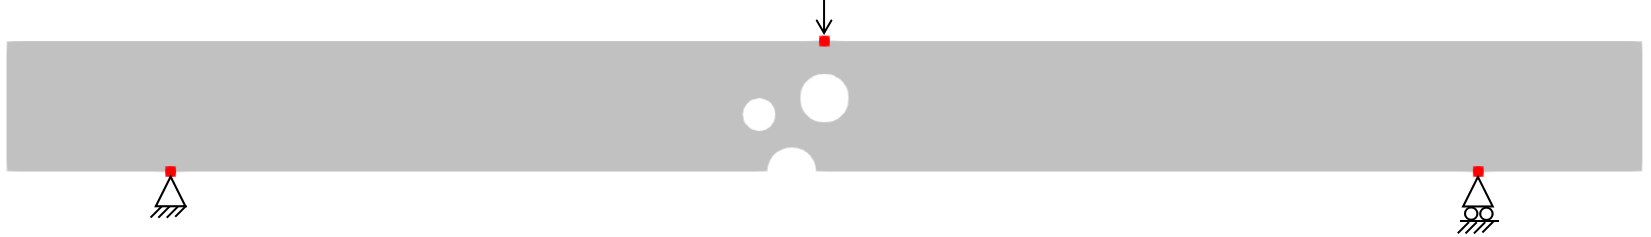
\includegraphics[width=\textwidth,scale=0.5]{Chapter5/figures/3pb/3pb_bc}
    \caption{}
  \end{subfigure}
  \begin{subfigure}[b]{0.9\textwidth}
    \centering
    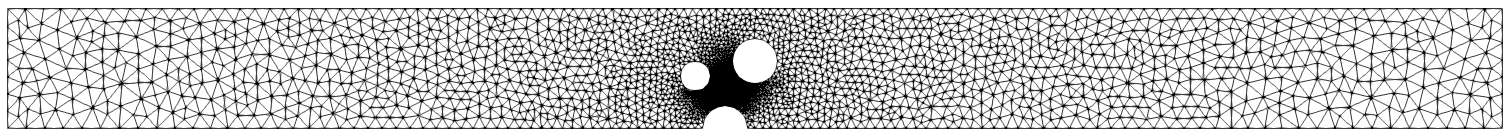
\includegraphics[width=\textwidth,scale=0.5]{Chapter5/figures/3pb/3pb_mesh}
    \caption{}
    \label{fig: Chapter5/3pb/3pb_mesh}
  \end{subfigure}
  \caption{(a) schematics of the three-point bending experiment and (b) the mesh. See \cite{kubik2019ductile} for a detailed drawing with dimensions. The specimen is assumed to have a fixed support and a roller support on the bottom, and a downward displacement is applied at the location of the top punch.}
  \label{fig: Chapter5/3pb/3pb}
\end{figure}


In the experiment, the crack surface first originates from the half cylindrical notch on the bottom of the specimen, and then grows to connect the notch to the bottom of the left smaller cylindrical hole. After a while, the second crack surface originates from the top of the left smaller hole and grows towards the middle of the upper free surface.

%%%%%%%%%%%%%%%%%%%%%%%%%%%%%%%%%%%%%%%%%%%%%%%%%%%%%%%%%%%%%%%%%%%%%%%%%%%%%%%%%%%%%%%%%%%
%%%%%%%%%%%%%%%%%%%%%%%%%%%%%%%%%%%%%%%%%%%%%%%%%%%%%%%%%%%%%%%%%%%%%%%%%%%%%%%%%%%%%%%%%%%
%%%%%%%%%%%%%%%%%%%%%%%%%%%%%%%%%%%%%%%%%%%%%%%%%%%%%%%%%%%%%%%%%%%%%%%%%%%%%%%%%%%%%%%%%%%
%%%%%%%%%%%%%%%%%%%%%%%%%%%%%%%%%%%%%%%%%%%%%%%%%%%%%%%%%%%%%%%%%%%%%%%%%%%%%%%%%%%%%%%%%%%
%%%%%%%%%%%%%%%%%%%%%%%%%%%%%%%%%%%%%%%%%%%%%%%%%%%%%%%%%%%%%%%%%%%%%%%%%%%%%%%%%%%%%%%%%%%
%%%%%%%%%%%%%%%%%%%%%%%%%%%%%%%%%%%%%%%%%%%%%%%%%%%%%%%%%%%%%%%%%%%%%%%%%%%%%%%%%%%%%%%%%%%
%%%%%%%%%%%%%%%%%%%%%%%%%%%%%%%%%%%%%%%%%%%%%%%%%%%%%%%%%%%%%%%%%%%%%%%%%%%%%%%%%%%%%%%%%%%
%%%%%%%%%%%%%%%%%%%%%%%%%%%%%%%%%%%%%%%%%%%%%%%%%%%%%%%%%%%%%%%%%%%%%%%%%%%%%%%%%%%%%%%%%%%
%%%%%%%%%%%%%%%%%%%%%%%%%%%%%%%%%%%%%%%%%%%%%%%%%%%%%%%%%%%%%%%%%%%%%%%%%%%%%%%%%%%%%%%%%%%
%%%%%%%%%%%%%%%%%%%%%%%%%%%%%%%%%%%%%%%%%%%%%%%%%%%%%%%%%%%%%%%%%%%%%%%%%%%%%%%%%%%%%%%%%%%
\subsubsection{Two-dimensional results}
\label{section: Chapter5/examples/3pb/2D}

First, we focus attention on the initiation and propagation of the first crack, i.e.\ the crack connecting the notch to the left smaller hole. The calculations are performed in two dimensions under plane-strain assumptions. The experimental crack path and the contours of the equivalent plastic strain are shown in \Cref{fig: Chapter5/3pb/plastic_strain}. Due to the nature of the linear crack geometric function, both the E-P-PD model and the E-P-D model has the same ductile response up to damage initiation: the equivalent plastic strain localizes around the middle of the bottom cylindrical notch, and two wakes of plastic deformation form at $\ang{45}$ angle towards the lower surfaces of the left smaller cylindrical hole and the right larger cylindrical hole.

\begin{figure}[!htb]
  \centering
  \begin{subfigure}[b]{0.3\textwidth}
    \centering
    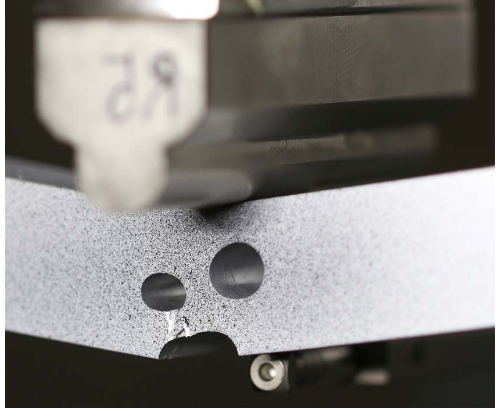
\includegraphics[width=\textwidth,scale=0.5]{Chapter5/figures/3pb/real_crack}
    \caption{}
  \end{subfigure}
  \hspace{0.1\textwidth}
  \begin{subfigure}[b]{0.35\textwidth}
    \centering
    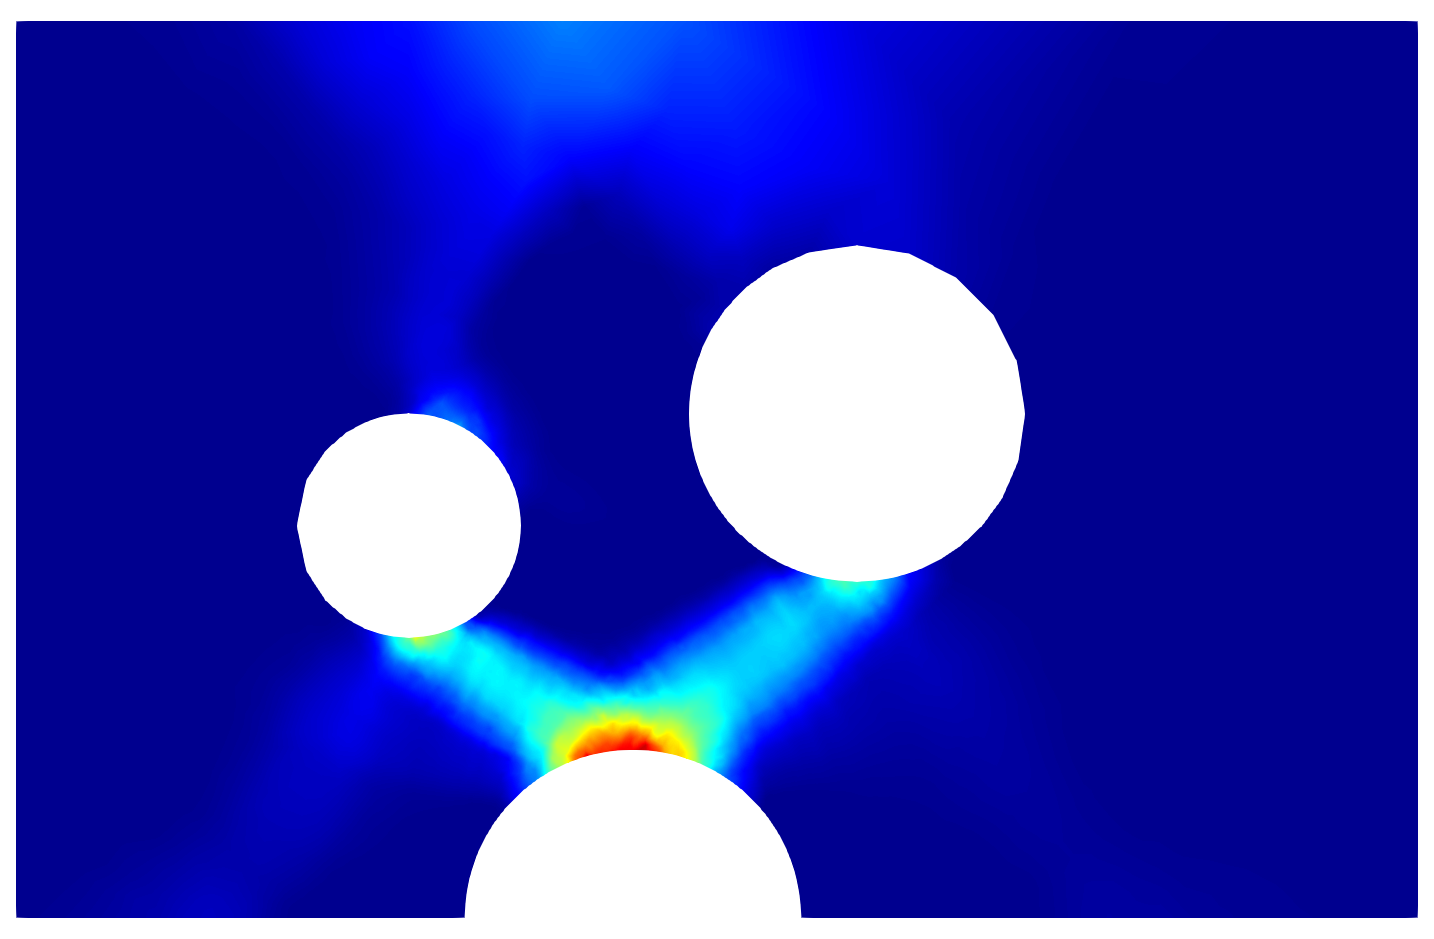
\includegraphics[width=\textwidth,scale=0.5]{Chapter5/figures/3pb/ep}
    \caption{}
  \end{subfigure}
  \begin{subfigure}[b]{0.06\textwidth}
    \centering
    \caption*{$\ep$}
    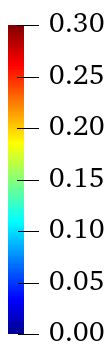
\includegraphics[width=\textwidth,scale=0.5]{Chapter5/figures/3pb/colorbar_ep}
    \vspace{1em}
  \end{subfigure}
  \label{fig: Chapter5/3pb/plastic_strain}
  \caption{(a) a picture of the experiment setup \cite{kubik2019ductile} and (b) the effective plastic strain prior to crack initiation.
  }
\end{figure}


It bears emphasis that this three-point bending experiment is particularly challenging for most E-P-D models because the crack trajectories will be qualitatively different in a brittle material and in a ductile material, and it is of common concern that a loosely coupled E-P-D model may fail to predict the correct crack trajectory. In fact, we show that it is important to include the coalescence dissipation to predict the correct crack path.

After damage initiation, crack paths predicted by the E-P-D model and the E-P-PD model differ. For the E-P-D model, the crack paths depend on the parameters chosen for the coalescence dissipation. The effective fracture toughness $\widehat{\Gc}(\ep;\beta, \varepsilon_0)$ decreases as the plastic strain $\ep$ increases following a decay characterized by $\beta$ and $\varepsilon_0$. In other words, the spatial variation of the effective fracture toughness conforms with the localization of the plastic strain.
The effect of $\beta$ and $\varepsilon_0$ are illustrated in \Cref{fig: Chapter5/3pb/2D_comparison_constant_beta,fig: Chapter5/3pb/2D_comparison_constant_e0}.

\begin{figure}[!htb]
  \centering
  \begin{subfigure}[b]{0.3\textwidth}
    \centering
    
\includegraphics[width=\textwidth,scale=0.5]{Chapter5/figures/3pb/beta_0.1_e0_0.8}
    \caption{$\varepsilon_0=0.8$}
  \end{subfigure}
  \begin{subfigure}[b]{0.3\textwidth}
    \centering
    
\includegraphics[width=\textwidth,scale=0.5]{Chapter5/figures/3pb/beta_0.1_e0_0.4}
    \caption{$\varepsilon_0=0.4$}
  \end{subfigure}
  \begin{subfigure}[b]{0.3\textwidth}
    \centering
    
\includegraphics[width=\textwidth,scale=0.5]{Chapter5/figures/3pb/beta_0.1_e0_0.2}
    \caption{$\varepsilon_0=0.2$}
  \end{subfigure}
  
  \begin{subfigure}[b]{0.3\textwidth}
    \centering
    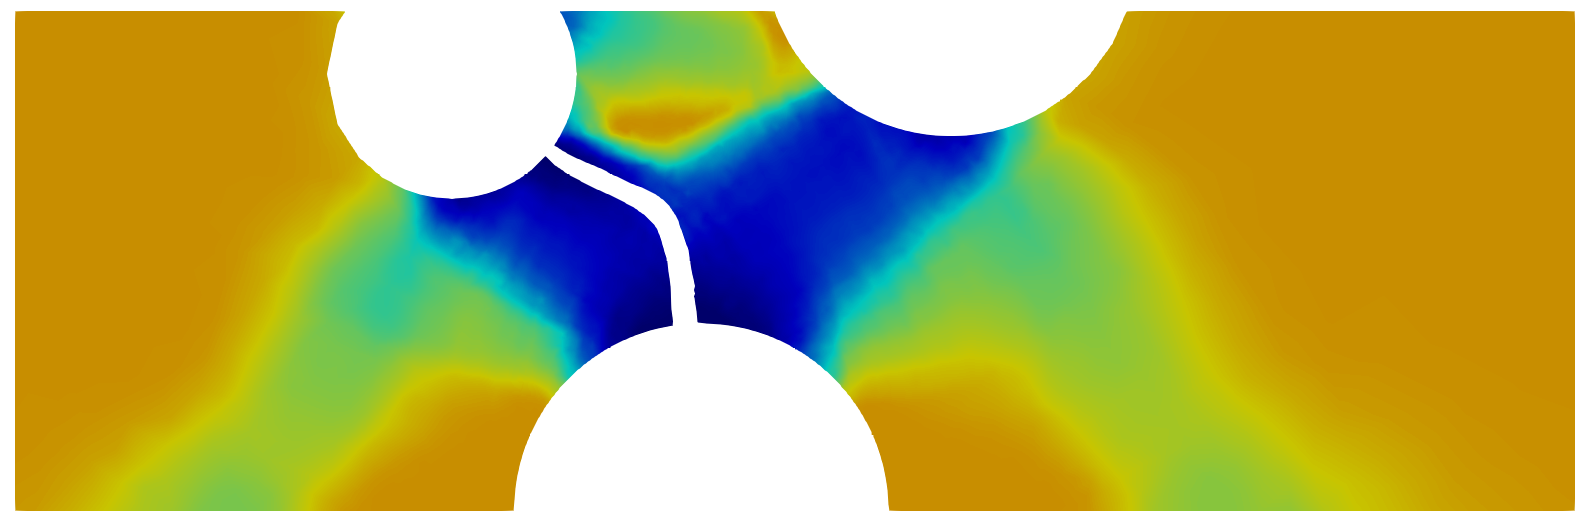
\includegraphics[width=\textwidth,scale=0.5]{Chapter5/figures/3pb/beta_0.1_e0_0.1}
    \caption{$\varepsilon_0=0.1$}
  \end{subfigure}
  \begin{subfigure}[b]{0.3\textwidth}
    \centering
    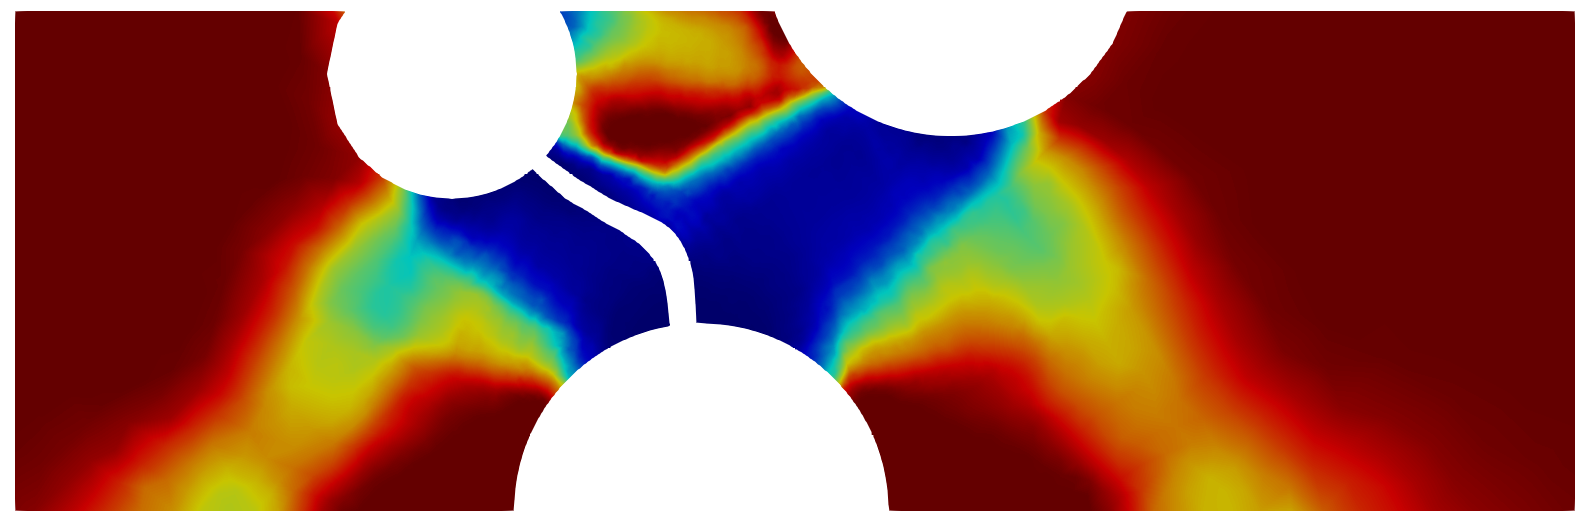
\includegraphics[width=\textwidth,scale=0.5]{Chapter5/figures/3pb/beta_0.1_e0_0.05}
    \caption{$\varepsilon_0=0.05$}
  \end{subfigure}
  \begin{subfigure}[b]{0.3\textwidth}
    \centering
    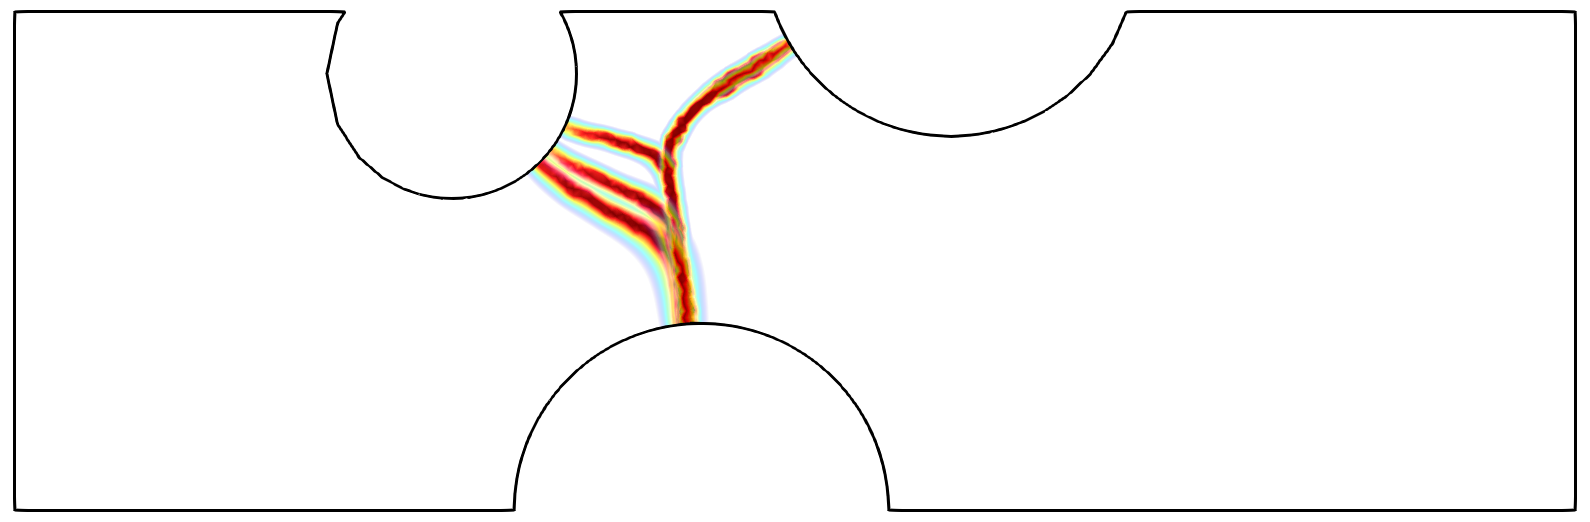
\includegraphics[width=\textwidth,scale=0.5]{Chapter5/figures/3pb/compare_beta_constant}
    \caption{}
  \end{subfigure}
  \caption[Comparison of crack paths for different values of $\epsilon_0$.]{(a-e) Contour plots of the effective fracture toughness $\widehat{\Gc}$ with $\beta=0.1$ and different values of $\varepsilon_0$, using the E-P-D model. The portion of the domain with $d > 0.8$ is removed to visualize the crack path. (f) Superposition of the damage contours. All contours are plotted on the reference configuration for the purpose of comparison.}
  \label{fig: Chapter5/3pb/2D_comparison_constant_beta}
\end{figure}


In \Cref{fig: Chapter5/3pb/2D_comparison_constant_beta}, $\beta$ is kept constant and the sensitivity of the fracture path to $\varepsilon_0$ is examined. Smaller values of $\varepsilon_0$ result in faster decay of the fracture toughness as the plastic strain increases. As a result, given the same amount of plastic strain, a smaller $\varepsilon_0$ leads to a higher spatial variation or ``contrast'' in the effective fracture toughness. When $\varepsilon_0 = 0.8$, the contrast is negligible, the effective fracture toughness is approximately homogeneous, and the crack propagates towards the right larger cylindrical hole. When $\varepsilon_0=0.05$, the contrast is high, the fracture toughness is degraded in regions with large plastic strain, and therefore the crack path largely follows the localization of the plastic strain.

Similar arguments hold in \Cref{fig: Chapter5/3pb/2D_comparison_constant_e0} where $\varepsilon_0$ is kept constant and the sensitivity of the fracture path to changes in $\beta$ is explored. When $\beta$ is small, the spatial ``contrast'' of the effective fracture toughness is high, and the crack path is affected by the localization of the plastic strain.

\begin{figure}[!htb]
  \centering
  \begin{subfigure}[b]{0.3\textwidth}
    \centering
    
\includegraphics[width=\textwidth,scale=0.5]{Chapter5/figures/3pb/beta_1}
    \caption{$\beta=1$}
  \end{subfigure}
  \begin{subfigure}[b]{0.3\textwidth}
    \centering
    
\includegraphics[width=\textwidth,scale=0.5]{Chapter5/figures/3pb/beta_0.8}
    \caption{$\beta=0.8$}
  \end{subfigure}
  \begin{subfigure}[b]{0.3\textwidth}
    \centering
    
\includegraphics[width=\textwidth,scale=0.5]{Chapter5/figures/3pb/beta_0.6}
    \caption{$\beta=0.6$}
  \end{subfigure}
  
  \begin{subfigure}[b]{0.3\textwidth}
    \centering
    
\includegraphics[width=\textwidth,scale=0.5]{Chapter5/figures/3pb/beta_0.4}
    \caption{$\beta=0.4$}
  \end{subfigure}
  \begin{subfigure}[b]{0.3\textwidth}
    \centering
    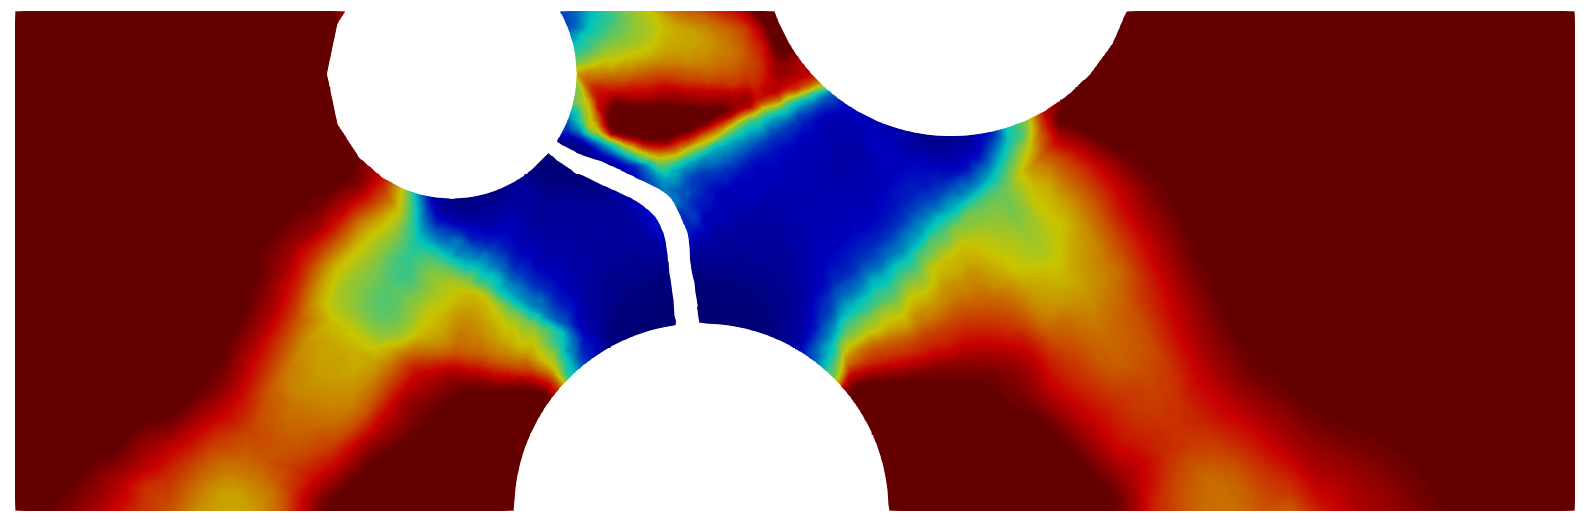
\includegraphics[width=\textwidth,scale=0.5]{Chapter5/figures/3pb/beta_0.2}
    \caption{$\beta=0.2$}
  \end{subfigure}
  \begin{subfigure}[b]{0.3\textwidth}
    \centering
    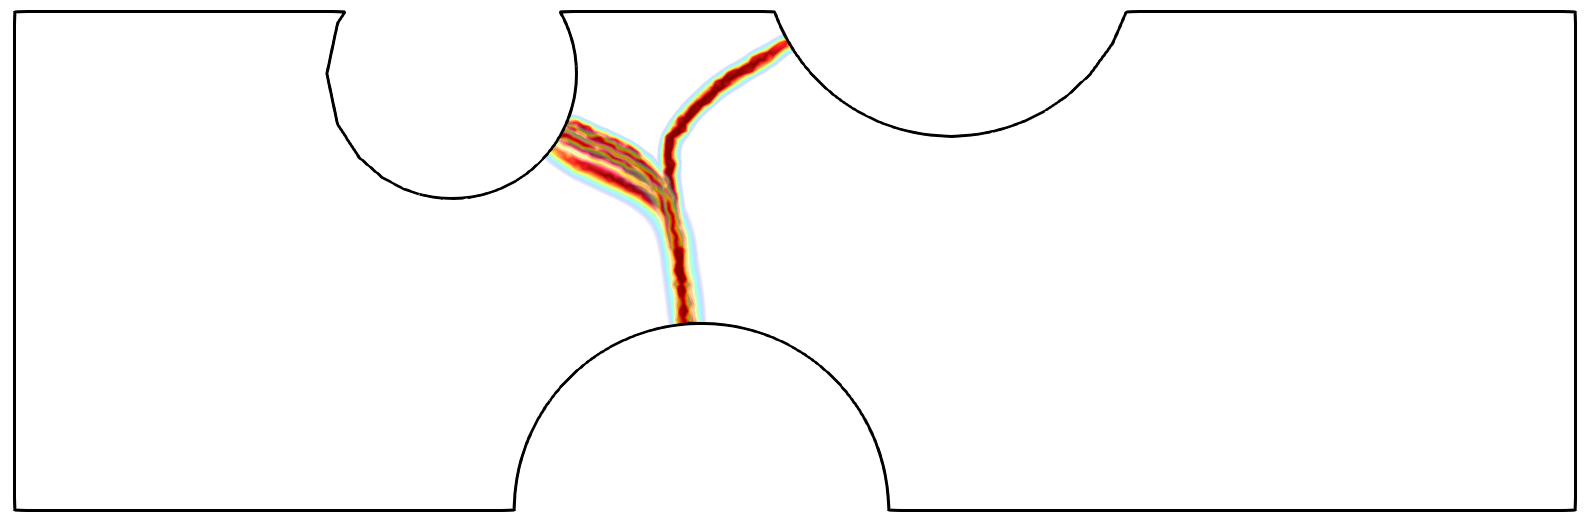
\includegraphics[width=\textwidth,scale=0.5]{Chapter5/figures/3pb/compare_e0_constant}
    \caption{}
  \end{subfigure}
  \caption{(a-e) Contour plots of the effective fracture toughness $\widehat{\Gc}$ with $\varepsilon_0=0.05$ and different values of $\beta$. Domain with $d > 0.8$ is removed to visualize the crack path. (f) Superposition of the damage contours. All contours are plotted on the reference configuration for the purpose of comparision.}
  \label{fig: Chapter5/3pb/2D_comparison_constant_e0}
\end{figure}


For the E-P-PD model, due to the strong coupling between plasticity and fracture, the crack path follows the localization of the plastic strain, and the plastic strain keeps increasing around the crack surface.  The resulting equivalent plastic strain and crack path in this case are shown in \Cref{fig: tpb-2d-eppd}.

\begin{figure}[htb!]
  \centering
  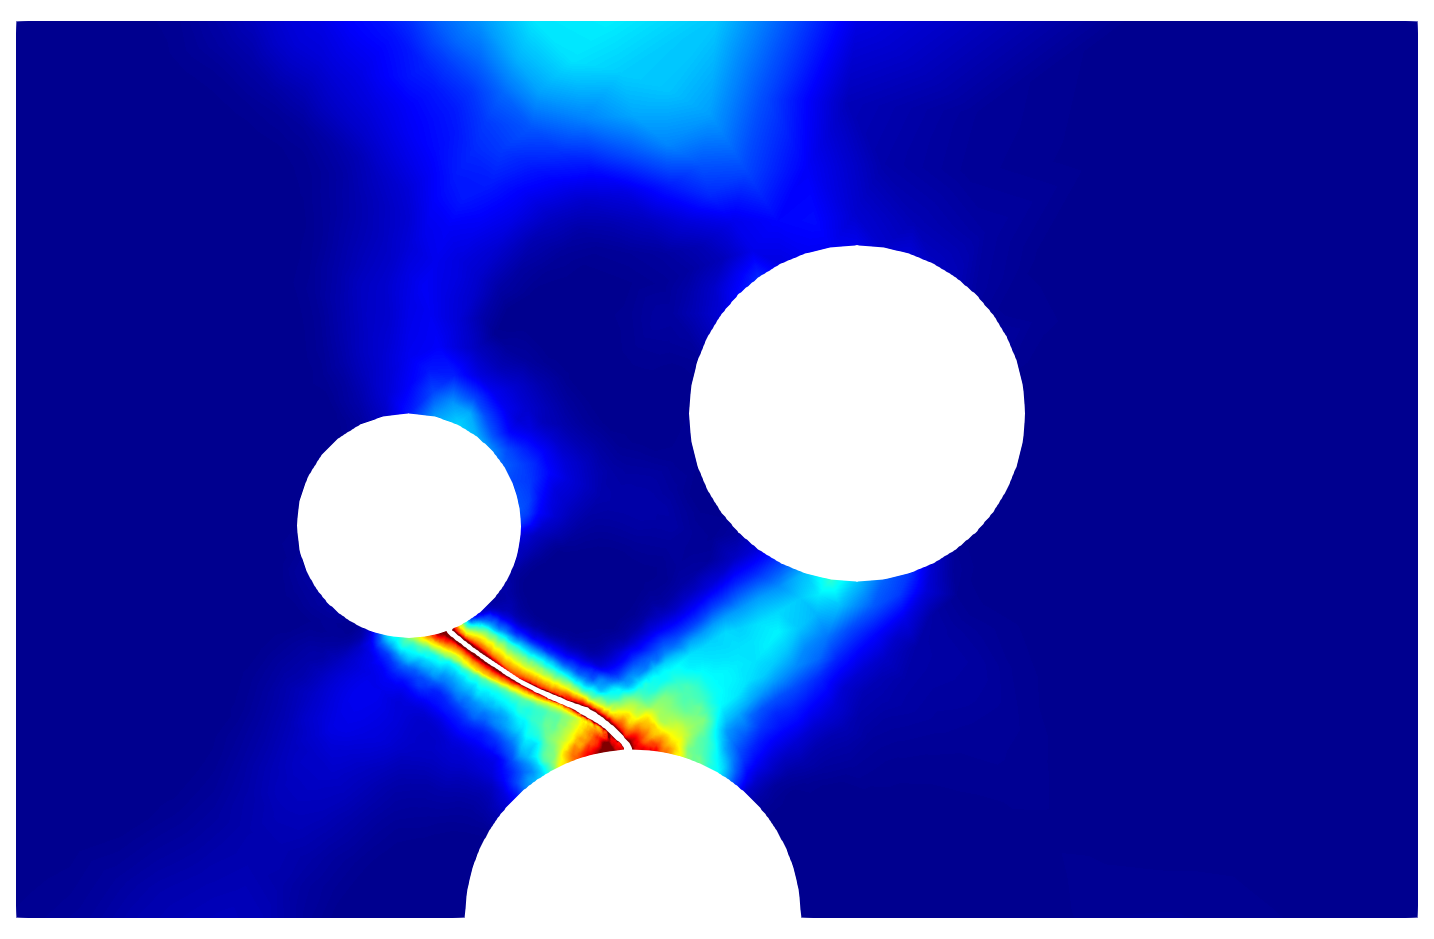
\includegraphics[width=0.3\textwidth,scale=0.5]{Chapter5/figures/3pb/2D_EPPD}
  \caption{Contour of the equivalent plastic strain obtained using the E-P-PD model. Domain with $d > 0.8$ is removed to visualize the crack path.}
  \label{fig: tpb-2d-eppd}
\end{figure}

\begin{remark}
  \vspace{-0.5em}
  In order to properly resolve the phase-field regularization length $l = \SI{0.01}{\milli\meter}$ for the E-P-PD model, a fairly small element size has to be used, resulting in a system with approximately 12 million degrees of freedom for this two-dimensional problem. In contrast, only 147,772 degrees of freedom were used for the E-P-D model.
\end{remark}

%%%%%%%%%%%%%%%%%%%%%%%%%%%%%%%%%%%%%%%%%%%%%%%%%%%%%%%%%%%%%%%%%%%%%%%%%%%%%%%%%%%%%%%%%%%
%%%%%%%%%%%%%%%%%%%%%%%%%%%%%%%%%%%%%%%%%%%%%%%%%%%%%%%%%%%%%%%%%%%%%%%%%%%%%%%%%%%%%%%%%%%
%%%%%%%%%%%%%%%%%%%%%%%%%%%%%%%%%%%%%%%%%%%%%%%%%%%%%%%%%%%%%%%%%%%%%%%%%%%%%%%%%%%%%%%%%%%
%%%%%%%%%%%%%%%%%%%%%%%%%%%%%%%%%%%%%%%%%%%%%%%%%%%%%%%%%%%%%%%%%%%%%%%%%%%%%%%%%%%%%%%%%%%
%%%%%%%%%%%%%%%%%%%%%%%%%%%%%%%%%%%%%%%%%%%%%%%%%%%%%%%%%%%%%%%%%%%%%%%%%%%%%%%%%%%%%%%%%%%
%%%%%%%%%%%%%%%%%%%%%%%%%%%%%%%%%%%%%%%%%%%%%%%%%%%%%%%%%%%%%%%%%%%%%%%%%%%%%%%%%%%%%%%%%%%
%%%%%%%%%%%%%%%%%%%%%%%%%%%%%%%%%%%%%%%%%%%%%%%%%%%%%%%%%%%%%%%%%%%%%%%%%%%%%%%%%%%%%%%%%%%
%%%%%%%%%%%%%%%%%%%%%%%%%%%%%%%%%%%%%%%%%%%%%%%%%%%%%%%%%%%%%%%%%%%%%%%%%%%%%%%%%%%%%%%%%%%
%%%%%%%%%%%%%%%%%%%%%%%%%%%%%%%%%%%%%%%%%%%%%%%%%%%%%%%%%%%%%%%%%%%%%%%%%%%%%%%%%%%%%%%%%%%
%%%%%%%%%%%%%%%%%%%%%%%%%%%%%%%%%%%%%%%%%%%%%%%%%%%%%%%%%%%%%%%%%%%%%%%%%%%%%%%%%%%%%%%%%%%
\subsubsection{Three-dimensional results}
\label{section: Chapter5/examples/3pb/3D}

With a qualitative understanding of the predicted trajectory of the first crack, a subset of the calibrated E-P-D models are now used in three-dimensional simulations of the three-point bending experiment.   The calculated load-deflection curves are compared to experimental measurements.

\begin{figure}[htb!]
  \centering
  \begin{subfigure}{0.45\textwidth}
    \centering
    \tikzsetnextfilenamesafe{Chapter5/3pb/load_deflection/constant_beta}
    \begin{tikzpicture}
      \begin{axis}[
          colormap/jet,
          cycle list={[of colormap,samples of colormap=4]},
          width=\textwidth,
          height=\textwidth,
          xmin=0,xmax=25,
          ymin=0,
          xlabel=deflection(\SI{}{\milli\meter}),ylabel=load(\SI{}{\kilo\newton}),
          scaled y ticks=false,
          xticklabel style={
              /pgf/number format/fixed,
              /pgf/number format/precision=2
            },
          legend style={
              at={(0.95,0.95)},
              anchor=north east,
              nodes={scale=0.8, transform shape},
              fill=white,
              fill opacity=0.8,
              draw opacity=1,
              text opacity=1,
              cells={align=left}
            },
          legend cell align={left},
          every axis plot/.append style={thick, no marks}
        ]
        \addplot [black,dashed] table[x expr=\thisrowno{0},y expr=\thisrowno{1}/1000,col sep=comma]{Chapter5/data/3pb/experiment1.csv};
        \addplot [black,dashdotted] table[x expr=\thisrowno{0},y expr=\thisrowno{1}/1000,col sep=comma]{Chapter5/data/3pb/experiment2.csv};
        \addplot table[x expr=\thisrowno{0},y expr=\thisrowno{1}/1000,col sep=comma]{Chapter5/data/3pb/force_disp_beta_0.1_e0_0.05.csv};
        \addplot table[x expr=\thisrowno{0},y expr=\thisrowno{1}/1000,col sep=comma]{Chapter5/data/3pb/force_disp_beta_0.1_e0_0.1.csv};
        \addplot table[x expr=\thisrowno{0},y expr=\thisrowno{1}/1000,col sep=comma]{Chapter5/data/3pb/force_disp_beta_0.1_e0_0.2.csv};
        \legend{experiment 1, experiment 2, $\varepsilon_0 = 0.05$, $\varepsilon_0 = 0.1$, $\varepsilon_0 = 0.2$}
      \end{axis}
    \end{tikzpicture}
    \caption{$\beta = 0.1$ and different values of $\varepsilon_0$}
    \label{fig: Chapter5/3pb/load_deflection/constant_beta}
  \end{subfigure}
  \begin{subfigure}{0.45\textwidth}
    \centering
    \tikzsetnextfilenamesafe{Chapter5/3pb/load_deflection/constant_e0}
    \begin{tikzpicture}
      \begin{axis}[
          colormap/jet,
          cycle list={[of colormap,samples of colormap=4]},
          width=\textwidth,
          height=\textwidth,
          xmin=0,xmax=25,
          ymin=0,
          xlabel=deflection(\SI{}{\milli\meter}),ylabel=load(\SI{}{\kilo\newton}),
          scaled y ticks=false,
          xticklabel style={
              /pgf/number format/fixed,
              /pgf/number format/precision=2
            },
          legend style={
              at={(0.95,0.95)},
              anchor=north east,
              nodes={scale=0.8, transform shape},
              fill=white,
              fill opacity=0.8,
              draw opacity=1,
              text opacity=1,
              cells={align=left}
            },
          legend cell align={left},
          every axis plot/.append style={thick, no marks}
        ]
        \addplot [black,dashed] table[x expr=\thisrowno{0},y expr=\thisrowno{1}/1000,col sep=comma]{Chapter5/data/3pb/experiment1.csv};
        \addplot [black,dashdotted] table[x expr=\thisrowno{0},y expr=\thisrowno{1}/1000,col sep=comma]{Chapter5/data/3pb/experiment2.csv};
        \addplot table[x expr=\thisrowno{0},y expr=\thisrowno{1}/1000,col sep=comma]{Chapter5/data/3pb/force_disp_beta_0.2_e0_0.05.csv};
        \addplot table[x expr=\thisrowno{0},y expr=\thisrowno{1}/1000,col sep=comma]{Chapter5/data/3pb/force_disp_beta_0.4_e0_0.05.csv};
        \addplot table[x expr=\thisrowno{0},y expr=\thisrowno{1}/1000,col sep=comma]{Chapter5/data/3pb/force_disp_beta_0.6_e0_0.05.csv};
        \addplot table[x expr=\thisrowno{0},y expr=\thisrowno{1}/1000,col sep=comma]{Chapter5/data/3pb/force_disp_beta_0.8_e0_0.05.csv};
        \legend{experiment 1, experiment 2, $\beta = 0.2$, $\beta = 0.4$, $\beta = 0.6$, $\beta = 0.8$}
      \end{axis}
    \end{tikzpicture}
    \caption{$\varepsilon_0 = 0.05$ and different values of $\beta$}
    \label{fig: Chapter5/3pb/load_deflection/constant_e0}
  \end{subfigure}
  \caption{Comparison of load-deflection curves between simulations and experiments \cite{kubik2019ductile} for the 3D three-point bend experiment.}
  \label{fig: Chapter5/3pb/load_deflection}
\end{figure}


In \cite{kubik2019ductile}, experimental results are reported for two different trials of the three-point bending experiment, both using the same material, geometry, and etc.  Both of the experimental load-deflection curves are shown in \Cref{fig: Chapter5/3pb/load_deflection} for the sake of comparison to our simulation results. The experimental curves indicate an initial elastic-plastic response, followed by an abrupt drop in the load, subsequent force increase, and a final abrupt drop.  The two drops in the force-displacement data (occurring for both experiments) correspond to the nucleation and propagation of the crack surfaces, first from the bottom notch to the hole, then from the hole to the upper free surface.

In the experiments, the first load drop occurs at a deflection around $\SI{5.8}{\milli\meter}$ (experiment 1) and $\SI{5.3}{\milli\meter}$ (experiment 2), and the second load drop occurs at a deflection around $\SI{10.1}{\milli\meter}$ (experiment 1) and $\SI{10.7}{\milli\meter}$ (experiment 2).
In all load-deflection curves predicted by the model-based simulations, the first load drop occurs at a deflection of approximately  $\SI{5.3}{\milli\meter}$, which compares well to the experimental measurements.
However, the prediction of the nucleation and propagation of the second crack is sensitive to model parameters $\beta$ and $\varepsilon_0$. While $\beta = 0.1$ is kept constant (\Cref{fig: Chapter5/3pb/load_deflection/constant_beta}), larger $\varepsilon_0$ delays the nucleation of the second crack and leads to a steeper load drop.  While $\varepsilon_0 = 0.05$ is kept constant (\Cref{fig: Chapter5/3pb/load_deflection/constant_e0}), larger $\beta$ values accelerate the nucleation of the second crack, but the load drops at approximately the same rate.

The results shown in \Cref{fig: Chapter5/3pb/load_deflection} suggest that choosing $\varepsilon_0=0.2$ and $\beta=0.6$ might result in a force-displacement curve that best matches the experimental data (the combination $\beta=0.6$ and $\varepsilon_0=0.2$ yields a force-displacement response that is practically indistinguishable from those shown in \Cref{fig: Chapter5/3pb/force_disp/EPD_beta,fig: Chapter5/3pb/force_disp/EPD_e0}).
We performed an additional simulation using this choice of these parameters, and the results are shown in \Cref{fig: Chapter5/3pb/load_deflection_tuned}. Indeed, the resulting simulation yields a force-displacement curve that is very close to the experimental result.   Importantly, we find that our model-based simulations yield a better comparison to the experimental load-displacement curves than the various damage models explored in \cite{kubik2019ductile}.

\begin{figure}[htb!]
  \centering
  \tikzsetnextfilenamesafe{Chapter5/3pb/load_deflection_tuned}
  \begin{tikzpicture}
    \begin{axis}[
        width=0.45\textwidth,
        height=0.45\textwidth,
        xmin=0,xmax=25,
        ymin=0,
        xlabel=deflection(\SI{}{\milli\meter}),ylabel=load(\SI{}{\kilo\newton}),
        scaled y ticks=false,
        xticklabel style={
            /pgf/number format/fixed,
            /pgf/number format/precision=2
          },
        legend style={
            at={(0.95,0.95)},
            anchor=north east,
            nodes={scale=0.8, transform shape},
            fill=white,
            fill opacity=0.8,
            draw opacity=1,
            text opacity=1,
            cells={align=left}
          },
        legend cell align={left},
        every axis plot/.append style={thick, no marks}
      ]
      \addplot [black,dashed] table[x expr=\thisrowno{0},y expr=\thisrowno{1}/1000,col sep=comma]{Chapter5/data/3pb/experiment1.csv};
      \addplot [black,dashdotted] table[x expr=\thisrowno{0},y expr=\thisrowno{1}/1000,col sep=comma]{Chapter5/data/3pb/experiment2.csv};
      \addplot [blue] table[x expr=\thisrowno{0},y expr=\thisrowno{1}/1000,col sep=comma]{Chapter5/data/3pb/force_disp_beta_0.6_e0_0.2.csv};
      \legend{experiment 1, experiment 2, $\beta = 0.6$ $\varepsilon_0 = 0.2$}
    \end{axis}
  \end{tikzpicture}
  \caption{Comparison of load-deflection curves between simulations and experiments \cite{kubik2019ductile} with tuned $\beta$ and $\varepsilon_0$.}
  \label{fig: Chapter5/3pb/load_deflection_tuned}
\end{figure}


While the load-deflection curves differ based on different choices of model parameters, the crack trajectory predictions are relatively insensitive to the model parameters. In the experiments (\Cref{fig: Chapter5/3pb/1234/experiment}), the crack nucleation and propagation can be divided into 4 stages. (I) The crack first nucleates around the center of the bottom notch and propagates through the thickness of the specimen. (II) Simultaneously the crack grows slant-wise towards the bottom of the smaller hole. (III) After a period of load increase, the second crack nucleates around the center of the top of the smaller hole and propagates through the thickness towards the free surfaces. (IV) Finally, the crack propagates towards the top free surface of the specimen.
The corresponding stages in the simulation are shown in \Cref{fig: Chapter5/3pb/1234/simulation_I,fig: Chapter5/3pb/1234/simulation_II,fig: Chapter5/3pb/1234/simulation_III,fig: Chapter5/3pb/1234/simulation_IV}.

\begin{figure}[!htb]
  \centering
  \begin{subfigure}{0.33\textwidth}
    \centering
    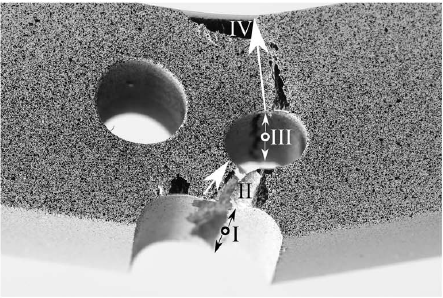
\includegraphics[width=\textwidth,scale=0.5]{Chapter5/figures/3pb/1234}
    \caption{experiment}
    \label{fig: Chapter5/3pb/1234/experiment}
  \end{subfigure}
  \hfill
  \begin{minipage}{0.6\textwidth}
    \begin{subfigure}{0.45\textwidth}
      \centering
      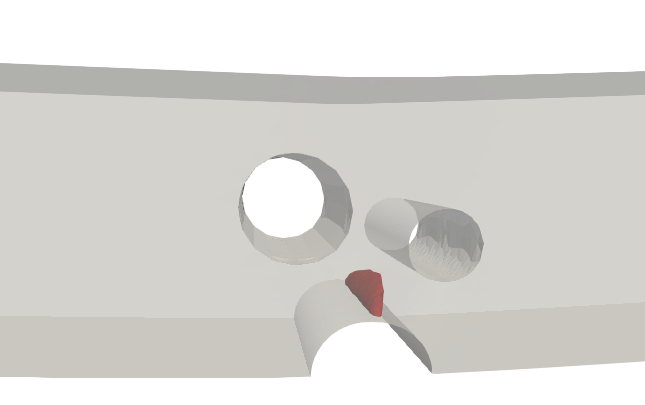
\includegraphics[width=\linewidth]{Chapter5/figures/3pb/I}
      \caption{stage I}
      \label{fig: Chapter5/3pb/1234/simulation_I}
    \end{subfigure}
    \begin{subfigure}{0.45\textwidth}
      \centering
      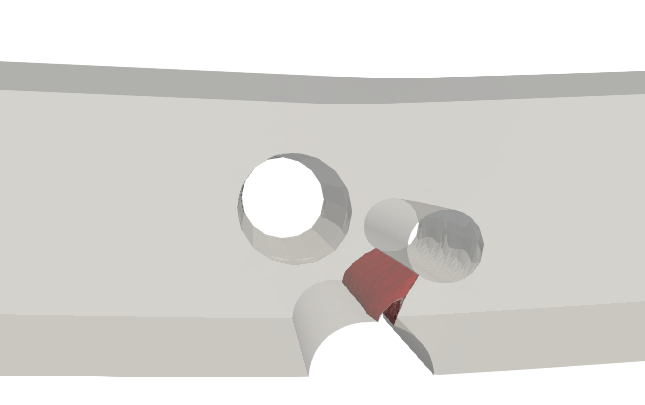
\includegraphics[width=\linewidth]{Chapter5/figures/3pb/II}
      \caption{stage II}
      \label{fig: Chapter5/3pb/1234/simulation_II}
    \end{subfigure}
    
    \begin{subfigure}{0.45\textwidth}
      \centering
      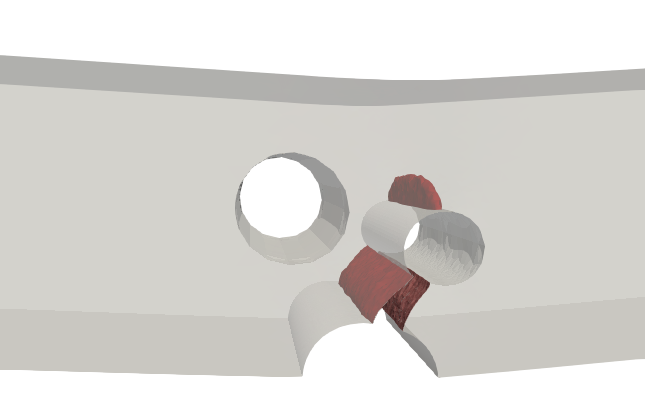
\includegraphics[width=\linewidth]{Chapter5/figures/3pb/III}
      \caption{stage III}
      \label{fig: Chapter5/3pb/1234/simulation_III}
    \end{subfigure}
    \begin{subfigure}{0.45\textwidth}
      \centering
      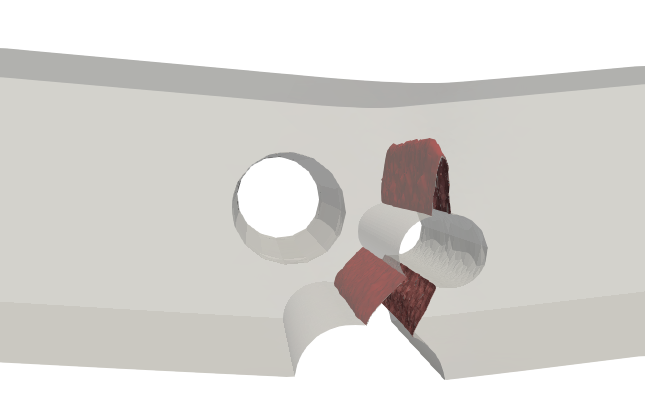
\includegraphics[width=\linewidth]{Chapter5/figures/3pb/IV}
      \caption{stage IV}
      \label{fig: Chapter5/3pb/1234/simulation_IV}
    \end{subfigure}
  \end{minipage}
  \caption[Comparison of crack paths between the experiment and the simulation.]{Comparison of crack paths between (a) the experiment \cite{kubik2019ductile} and (b-e) the simulation with $\beta = 0.6$ and $\varepsilon_0 = 0.2$. Iso-contours of $d=0.8$ are highlighted in red. }
  \label{fig: Chapter5/3pb/1234}
\end{figure}


The final crack surfaces obtained using $\beta = 0.6$ and $\varepsilon_0 = 0.2$ are shown in \Cref{fig: Chapter5/3pb/split_comparison}. In the experiments, ``shear lips'' (circled in red) occur close to the free surfaces of the specimen due to high stress-triaxility. Although such ``shear lips'' are not predicted by the E-P-D model used in this work, the larger-scale crack trajectories agree reasonably well with the experimental observations.

\begin{figure}[!htb]
  \centering
  \begin{subfigure}[b]{0.4\textwidth}
    \centering
    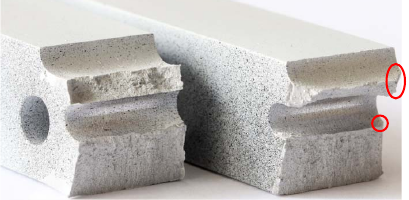
\includegraphics[width=\textwidth,scale=0.5]{Chapter5/figures/3pb/split_experiment}
    \caption{}
  \end{subfigure}
  \begin{subfigure}[b]{0.4\textwidth}
    \centering
    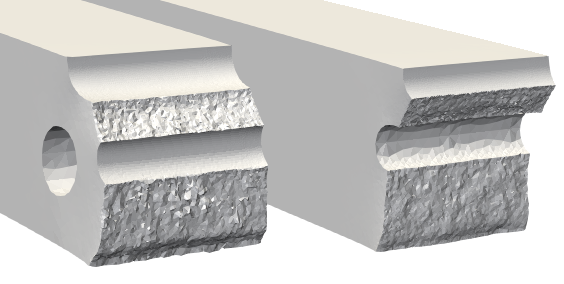
\includegraphics[width=\textwidth,scale=0.5]{Chapter5/figures/3pb/split}
    \caption{}
  \end{subfigure}
  \caption{Comparison of the final crack surfaces between (a) the experiment \cite{kubik2019ductile} and (b) the simulation ($\beta = 0.1$ and $\varepsilon_0 = 0.2$). ``Shear lips'' are circled in red. For comparison purposes, the computational domain is separated into two pieces by removing the domain within the $d \ge 0.8$ contour after complete failure.}
  \label{fig: Chapter5/3pb/split_comparison}
\end{figure}


%%%%%%%%%%%%%%%%%%%%%%%%%%%%%%%%%%%%%%%%%%%%%%%%%%%%%%%%%%%%%%%%%%%%%%%%%%%%%%%%%%%%%%%%%%%
%%%%%%%%%%%%%%%%%%%%%%%%%%%%%%%%%%%%%%%%%%%%%%%%%%%%%%%%%%%%%%%%%%%%%%%%%%%%%%%%%%%%%%%%%%%
%%%%%%%%%%%%%%%%%%%%%%%%%%%%%%%%%%%%%%%%%%%%%%%%%%%%%%%%%%%%%%%%%%%%%%%%%%%%%%%%%%%%%%%%%%%
%%%%%%%%%%%%%%%%%%%%%%%%%%%%%%%%%%%%%%%%%%%%%%%%%%%%%%%%%%%%%%%%%%%%%%%%%%%%%%%%%%%%%%%%%%%
%%%%%%%%%%%%%%%%%%%%%%%%%%%%%%%%%%%%%%%%%%%%%%%%%%%%%%%%%%%%%%%%%%%%%%%%%%%%%%%%%%%%%%%%%%%
%%%%%%%%%%%%%%%%%%%%%%%%%%%%%%%%%%%%%%%%%%%%%%%%%%%%%%%%%%%%%%%%%%%%%%%%%%%%%%%%%%%%%%%%%%%
%%%%%%%%%%%%%%%%%%%%%%%%%%%%%%%%%%%%%%%%%%%%%%%%%%%%%%%%%%%%%%%%%%%%%%%%%%%%%%%%%%%%%%%%%%%
%%%%%%%%%%%%%%%%%%%%%%%%%%%%%%%%%%%%%%%%%%%%%%%%%%%%%%%%%%%%%%%%%%%%%%%%%%%%%%%%%%%%%%%%%%%
%%%%%%%%%%%%%%%%%%%%%%%%%%%%%%%%%%%%%%%%%%%%%%%%%%%%%%%%%%%%%%%%%%%%%%%%%%%%%%%%%%%%%%%%%%%
%%%%%%%%%%%%%%%%%%%%%%%%%%%%%%%%%%%%%%%%%%%%%%%%%%%%%%%%%%%%%%%%%%%%%%%%%%%%%%%%%%%%%%%%%%%
\subsection{The Sandia Fracture Challange}
\label{section: Chapter5/examples/SFC}

Next, we examine the capabilities of the proposed E-P-D model by simulating an experiment from a Sandia Fracture Challenge \cite{boyce2014sandia}.  The specimen is composed of Al-5052 H34.  The hardening model is first calibrated against  tensile test data for a smooth round bar \cite{guo2013experimental}. The calibrated material properties and model constants are summarized in \Cref{tab: Chapter5/SFC}. Based on the calibrated tensile test results, the crack should initiate at a critical equivalent plastic strain of $\varepsilon^p_c = 0.8$. The fracture toughness $\Gc$ is then scaled accordingly, such that $\widehat{\Gc}$ matches experimental measurements.

\begin{table}[htb!]
  \small
  \centering
  \caption{Summary of the calibrated material properties and model parameters for the Sandia Fracture Challenge specimen}
  \begin{tabular}{r | c | c | c }
    \toprule
    Property/Parameter               & Symbol          & Value           & Unit                                       \\
    \midrule
    Bulk modulus                     & $K$             & \SI{6.495e4}{}  & \SI{}{\mega\pascal}                        \\
    Shear modulus                    & $G$             & \SI{2.4906e4}{} & \SI{}{\mega\pascal}                        \\
    \midrule
    Yield stress                     & $\sigma_y$      & 225             & \SI{}{\mega\pascal}                        \\
    Hardening modulus                & $H$             & 250             & \SI{}{\mega\pascal}                        \\
    \midrule
    Fracture toughness               & $\widehat{\Gc}$ & 13.6            & \SI{}{\milli\joule\per\square\milli\meter} \\
    Fracture dissipation coefficient & $\xi$           & 1               & nondim.                                    \\
    Critical fracture energy         & $\psi_c$        & 1               & \SI{}{\milli\joule\per\cubic\milli\meter}  \\
    Regularization length            & $l$             & 0.3             & \SI{}{\milli\meter}                        \\
    \midrule
    Interaction coefficient          & $\beta$         & 0.5             & nondim.                                    \\
    Characteristic plastic strain    & $\varepsilon_0$ & 0.1             & nondim.                                    \\
    \bottomrule
  \end{tabular}
  \label{tab: Chapter5/SFC}
\end{table}

The calibrated model is then applied to simulate crack initiation and growth in the specimen adopted for the Sandia Fracture Challenge. Drawings of the specimen with detailed dimensions are available in \cite{guo2013experimental,ambati2016phase}. The geometry and the mesh of the specimen is shown in \Cref{fig: Chapter5/SFC/schematics}. The three-dimensional geometry is discretized using tetrahedral elements (\texttt{TET10}). The mesh is locally refined near the round notch to sufficiently capture plastic and fracture localizations. It is assumed that the extension of the second crack is known a priori, and the region to the right of the middle hole is also refined to properly resolve the phase field. The resulting mesh consists of 10831 tetrahedra.

The specimen is loaded in tension via two pins that connect to the specimen through the circular holes whose centers coincide with nodes $A$ and $B$ in \Cref{fig: Chapter5/SFC/schematics}.  Rather than apply the loads to the boundaries of the holes or employ a contact algorithm with the pins, here we simplify the model by explicitly meshing the pins and assuming they are perfectly bonded to the specimen at the hole locations.  The material of the pins is    assumed to be elastic with moduli that match the specimen.

\begin{figure}[!htb]
  \centering
  \tikzsetnextfilenamesafe{Chapter5/SFC/schematics}
  \begin{tikzpicture}
    \node[inner sep=0] (mesh) at (0,0) {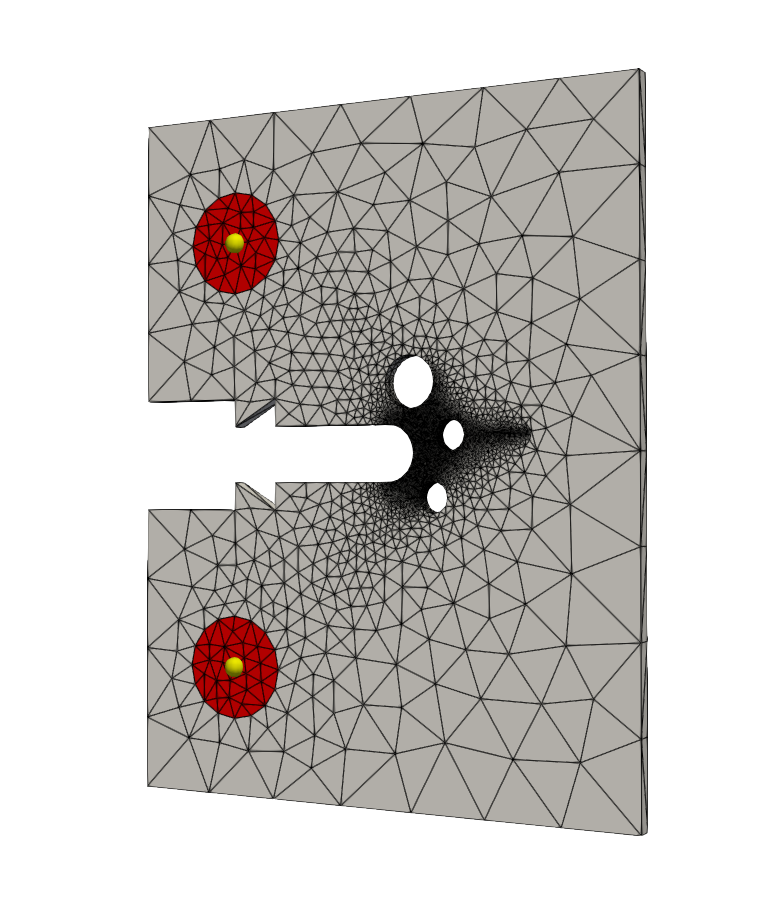
\includegraphics[width=0.3\textwidth,scale=0.5]{Chapter5/figures/SFC/mesh}};
    \coordinate (box_sw) at (-0.2, -0.6);
    \coordinate (box_nw) at (-0.2, 0.78);
    \coordinate (box_ne) at (1, 0.9);
    \coordinate (box_se) at (1, -0.65);
    
    \draw [blue] (box_sw) -- (box_nw);
    \draw [blue] (box_nw) -- (box_ne);
    \draw [blue] (box_ne) -- (box_se);
    \draw [blue] (box_se) -- (box_sw);
    
    \node[inner sep=0] (meshzoom) at (7,0) {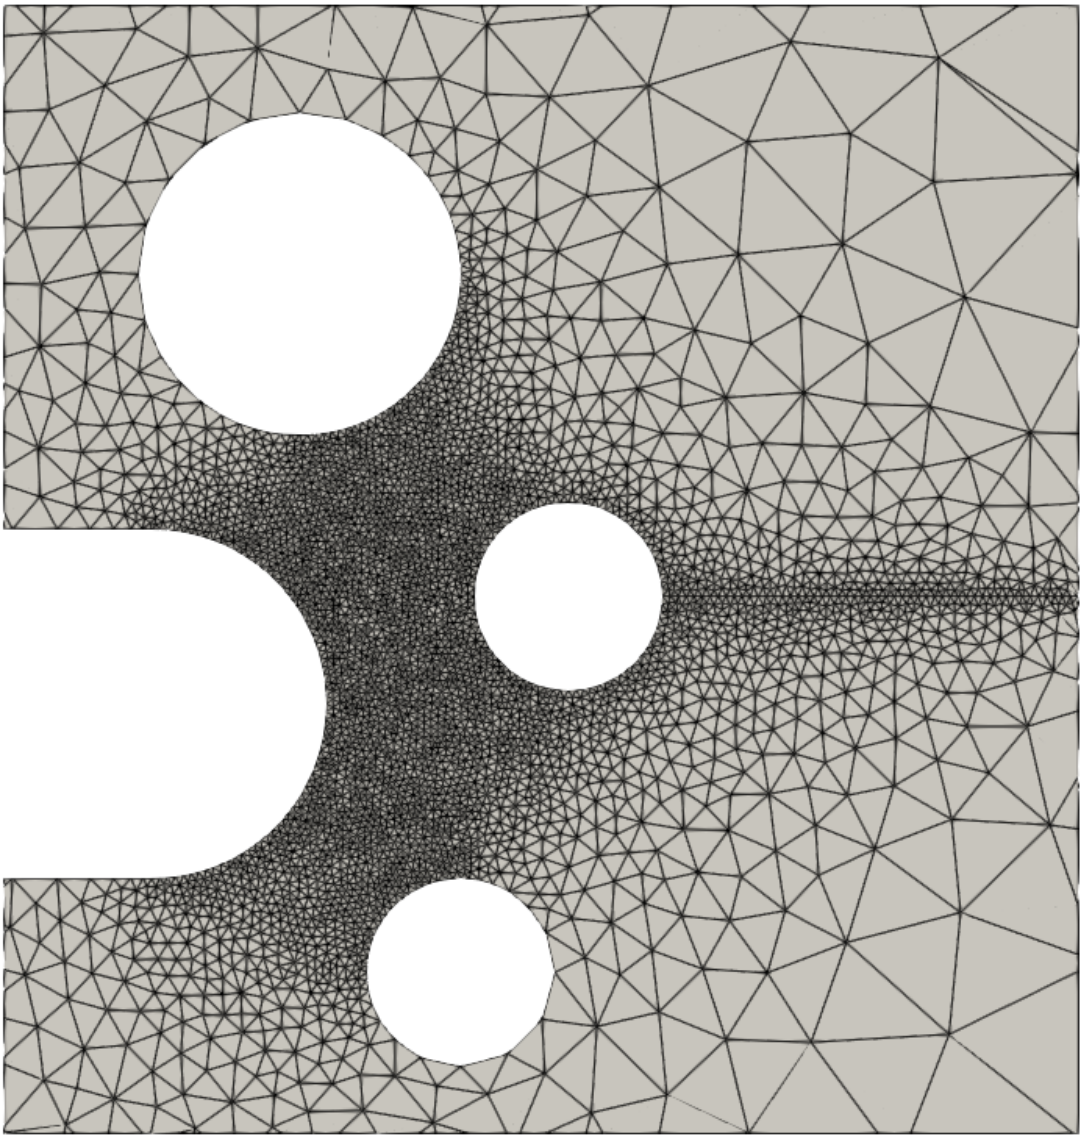
\includegraphics[width=0.3\textwidth,scale=0.5]{Chapter5/figures/SFC/meshzoom}};
    \node (boxzoom) at (meshzoom.south west) [draw,blue,thick,minimum width=0.3\textwidth,minimum height=147,anchor=south west] {};
    
    \draw (box_ne) -- (boxzoom.north west);
    \draw (box_se) -- (boxzoom.south west);
    
    \node (A) at (-1.2,1.6) [yellow] {\textbf{A}};
    \node (B) at (-1.2,-1.7) [yellow] {\textbf{B}};
  \end{tikzpicture}
  \caption[Sandia Fracture Challenge problem geometry and mesh, with zoomed-in view of the refined region.]{Sandia Fracture Challenge problem geometry and mesh, with zoomed-in view of the refined region. The specimen is loaded vertically with displacement control at lines of nodes A and B marked as yellow spheres.}
  \label{fig: Chapter5/SFC/schematics}
\end{figure}


The resulting force-displacement curves are shown in \Cref{fig: Chapter5/SFC/force_disp}. The response predicted by our proposed E-P-D model indicates an excellent agreement with the experimental measurements. Force-displacement curves from \cite{ambati2016phase} are also included for comparison.  The proposed E-P-D model clearly provides the best quantitative and qualitative match with the experiment.

Contour plots of the phase field $d$ are shown in \Cref{fig: Chapter5/SFC/d_1,fig: Chapter5/SFC/d_2,fig: Chapter5/SFC/d_3}. The first crack nucleates on the left side of the middle hole, and then connects with the round notch. After a while, the second crack nucleates on the right side of the middle hole and propagates to the right, with a nearly horizontal orientation.
The active part of the strain energy is shown in \Cref{fig: Chapter5/SFC/We_1,fig: Chapter5/SFC/We_2,fig: Chapter5/SFC/We_3}, where the stress concentration at the crack tips and a stress release after the first crack can be clearly observed.
The plastic energy is shown in \Cref{fig: Chapter5/SFC/Wp_1,fig: Chapter5/SFC/Wp_2,fig: Chapter5/SFC/Wp_3}, and the coalescence degradation is shown in \Cref{fig: Chapter5/SFC/gc_1,fig: Chapter5/SFC/gc_2,fig: Chapter5/SFC/gc_3}. The fracture toughness is substantially degraded in the regions with high plastic localization.

\begin{figure}[!htb]
  \centering
  \tikzsetnextfilenamesafe{Chapter5/SFC/force_disp}
  \begin{tikzpicture}
    \begin{axis}[
        cycle list name=exotic,
        width=0.65\textwidth,
        height=0.4\textwidth,
        xmin=0,xmax=7,
        ymin=0,
        xlabel=displacement(\SI{}{\milli\meter}),ylabel=force(\SI{}{\kilo\newton}),
        scaled y ticks=false,
        xticklabel style={
            /pgf/number format/fixed,
            /pgf/number format/precision=2
          },
        legend style={
            at={(0.1,0.05)},
            anchor=south west,
            nodes={scale=0.6, transform shape},
            fill=white,
            fill opacity=0.8,
            draw opacity=1,
            text opacity=1,
            cells={align=left}
          },
        legend cell align={left},
        every axis plot/.append style={thick}
      ]
      \addplot +[mark=none,black,dashed] table[x expr=\thisrowno{0},y expr=\thisrowno{1}/1000,col sep=comma]{Chapter5/data/SFC/experiment.csv};
      \addplot +[mark=none] table[x expr=\thisrowno{0},y expr=\thisrowno{1}/1000,col sep=comma]{Chapter5/data/SFC/force_disp.csv};
      \addplot +[mark=none] table[x expr=\thisrowno{0},y expr=\thisrowno{1}/1000,col sep=comma]{Chapter5/data/SFC/force_disp_lorenzis_1.csv};
      \addplot +[mark=none] table[x expr=\thisrowno{0},y expr=\thisrowno{1}/1000,col sep=comma]{Chapter5/data/SFC/force_disp_lorenzis_2.csv};
      \legend{experiment,proposed E-P-D model,prediction with $m=1$ from Ambati et al.,prediction with $m=2$ from Ambati et al.}
    \end{axis}
  \end{tikzpicture}
  \caption{ The force displacement curves from the experiment and the numerical simulations for the Sandia Fracture Challenge. }
  \label{fig: Chapter5/SFC/force_disp}
\end{figure}

\begin{figure}[!htbp]
  \centering
  \begin{subfigure}{0.2\textwidth}
    \centering
    
\includegraphics[width=\textwidth,scale=0.5]{Chapter5/figures/SFC/d_1}
    \caption{$u = \SI{2.87}{\milli\meter}$}
    \label{fig: Chapter5/SFC/d_1}
  \end{subfigure}
  \hspace{0.03\textwidth}
  \begin{subfigure}{0.2\textwidth}
    \centering
    
\includegraphics[width=\textwidth,scale=0.5]{Chapter5/figures/SFC/d_2}
    \caption{$u = \SI{5.28}{\milli\meter}$}
    \label{fig: Chapter5/SFC/d_2}
  \end{subfigure}
  \hspace{0.03\textwidth}
  \begin{subfigure}{0.2\textwidth}
    \centering
    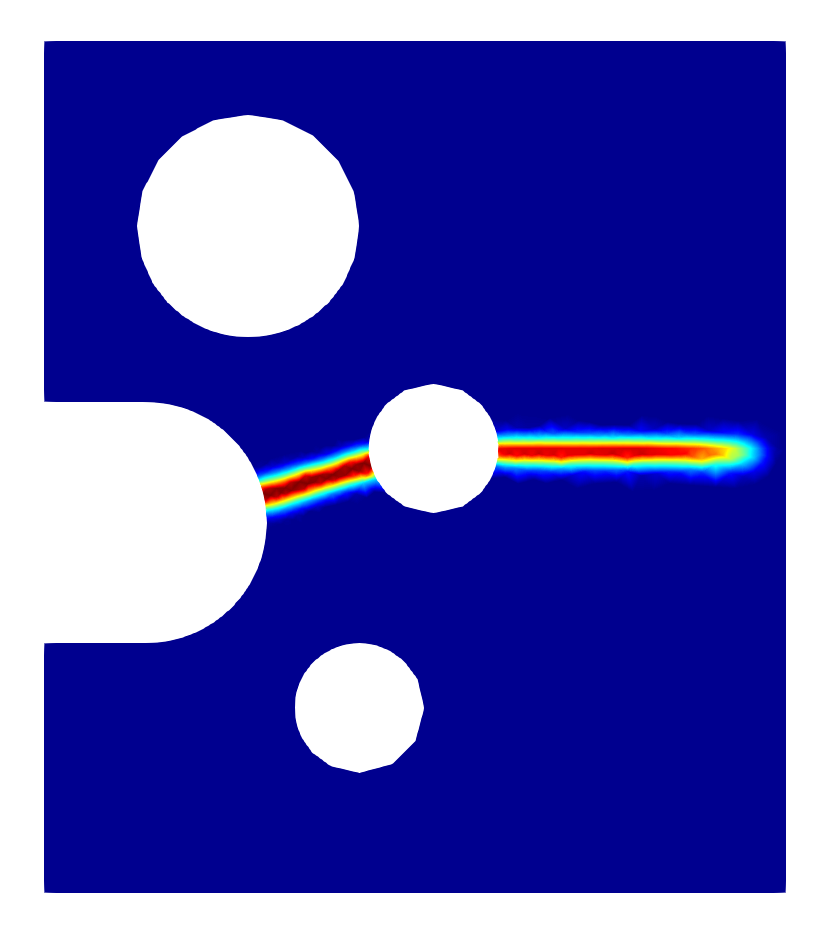
\includegraphics[width=\textwidth,scale=0.5]{Chapter5/figures/SFC/d_3}
    \caption{$u = \SI{6.81}{\milli\meter}$}
    \label{fig: Chapter5/SFC/d_3}
  \end{subfigure}
  \begin{subfigure}{0.05\textwidth}
    \centering
    \caption*{$d$}
    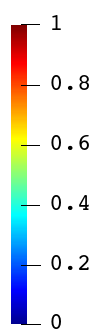
\includegraphics[width=\textwidth,scale=0.5]{Chapter5/figures/SFC/colorbar_d_vertical}
    \vspace{1em}
  \end{subfigure}
  
  \begin{subfigure}{0.2\textwidth}
    \centering
    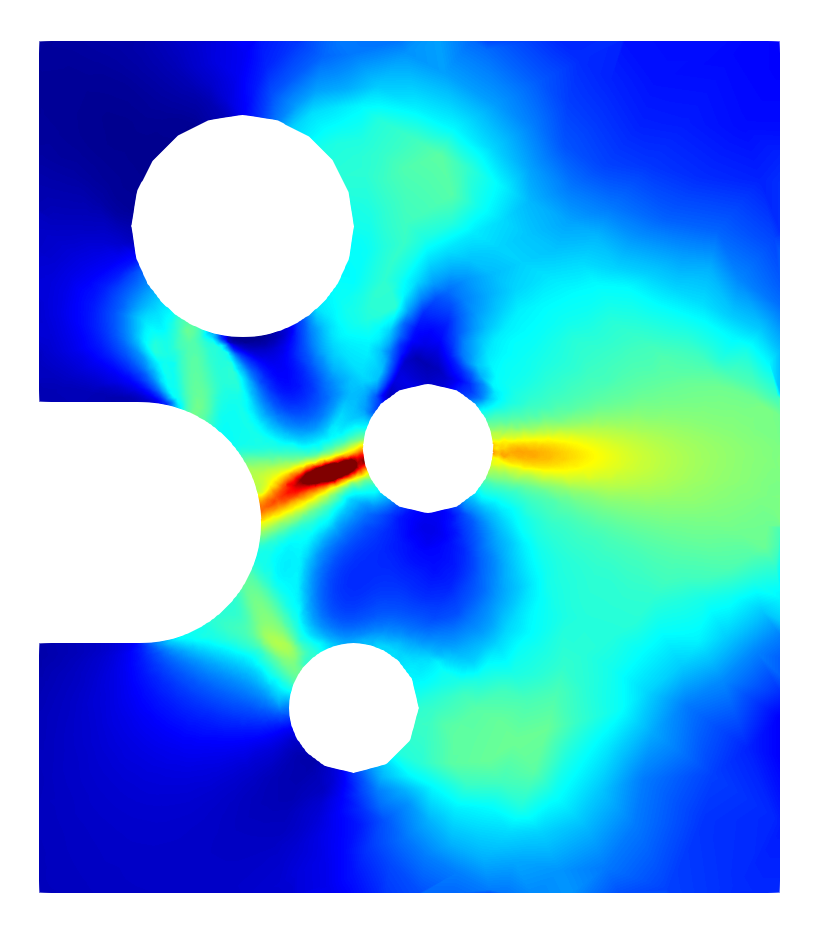
\includegraphics[width=\textwidth,scale=0.5]{Chapter5/figures/SFC/E_el_1}
    \caption{$u = \SI{2.87}{\milli\meter}$}
    \label{fig: Chapter5/SFC/We_1}
  \end{subfigure}
  \hspace{0.03\textwidth}
  \begin{subfigure}{0.2\textwidth}
    \centering
    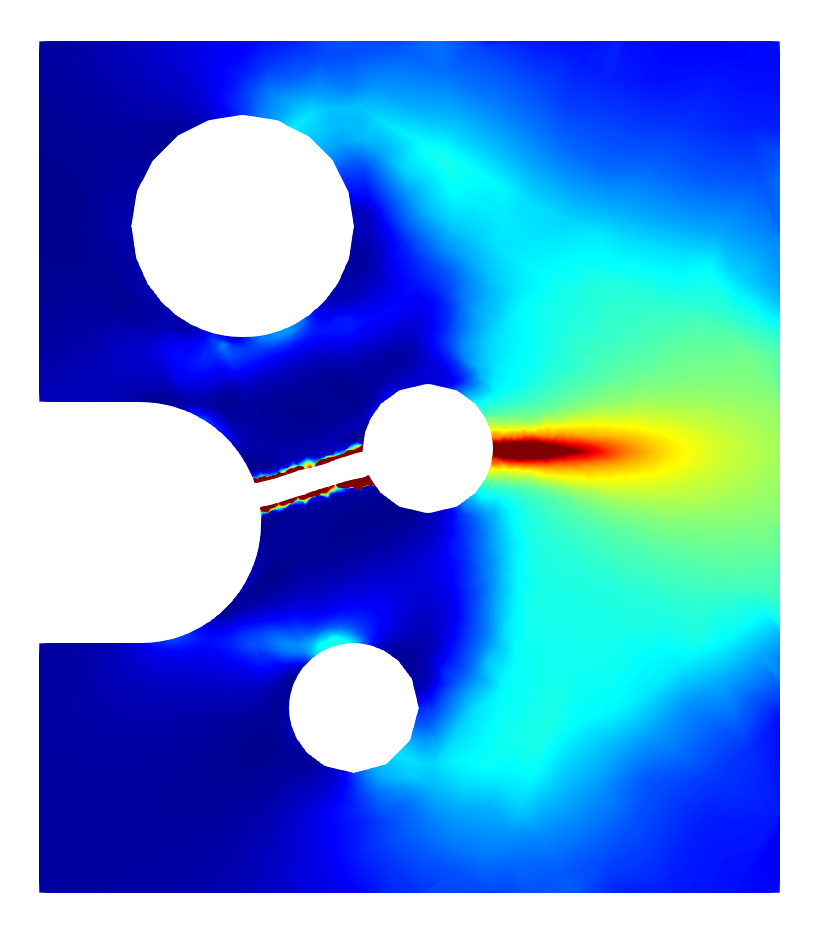
\includegraphics[width=\textwidth,scale=0.5]{Chapter5/figures/SFC/E_el_2}
    \caption{$u = \SI{5.28}{\milli\meter}$}
    \label{fig: Chapter5/SFC/We_2}
  \end{subfigure}
  \hspace{0.03\textwidth}
  \begin{subfigure}{0.2\textwidth}
    \centering
    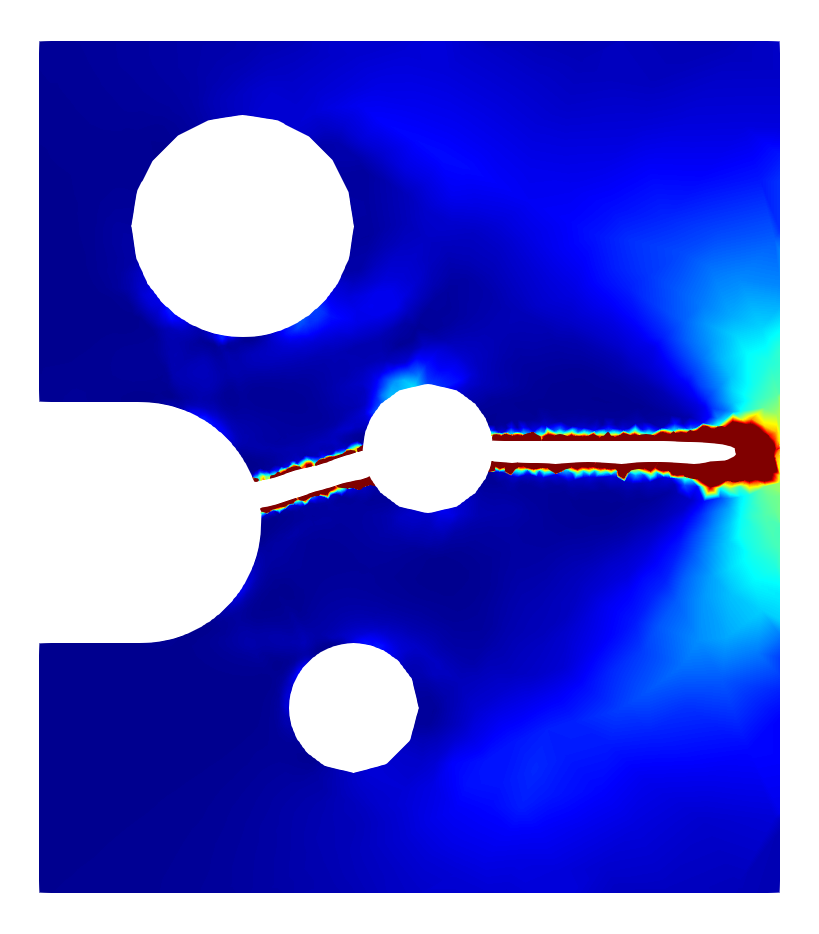
\includegraphics[width=\textwidth,scale=0.5]{Chapter5/figures/SFC/E_el_3}
    \caption{$u = \SI{6.81}{\milli\meter}$}
    \label{fig: Chapter5/SFC/We_3}
  \end{subfigure}
  \begin{subfigure}{0.05\textwidth}
    \centering
    \caption*{$\psi^e$}
    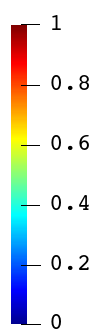
\includegraphics[width=\textwidth,scale=0.5]{Chapter5/figures/SFC/colorbar_We_vertical}
    \vspace{1em}
  \end{subfigure}
  
  \begin{subfigure}{0.2\textwidth}
    \centering
    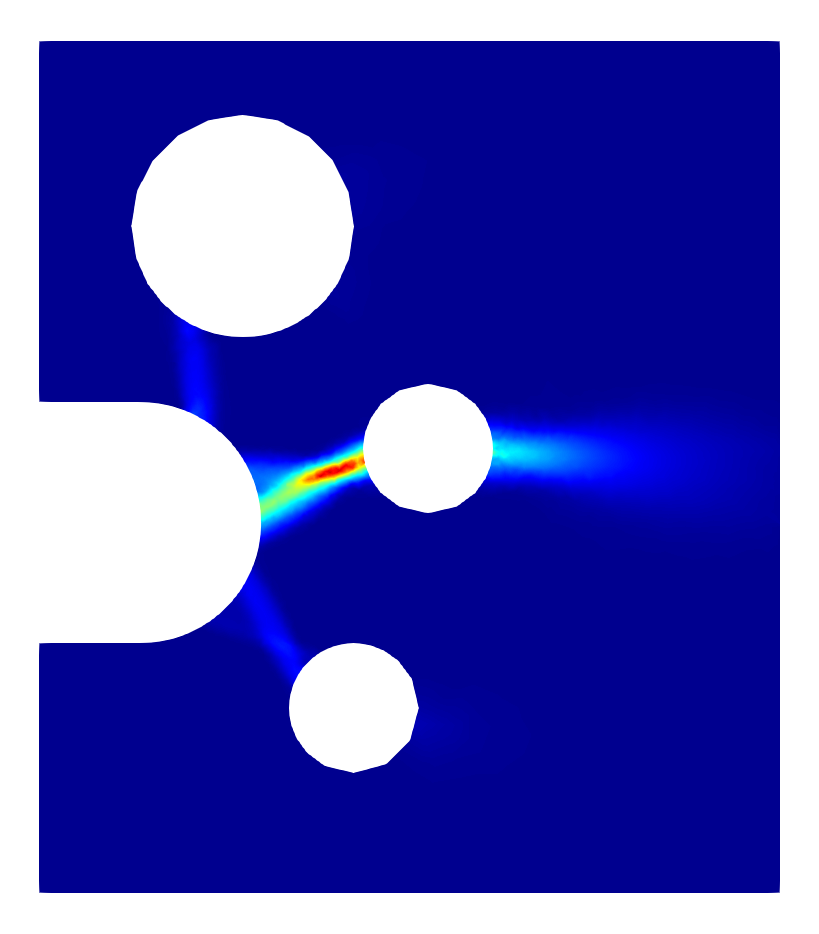
\includegraphics[width=\textwidth,scale=0.5]{Chapter5/figures/SFC/W_pl_1}
    \caption{$u = \SI{2.87}{\milli\meter}$}
    \label{fig: Chapter5/SFC/Wp_1}
  \end{subfigure}
  \hspace{0.03\textwidth}
  \begin{subfigure}{0.2\textwidth}
    \centering
    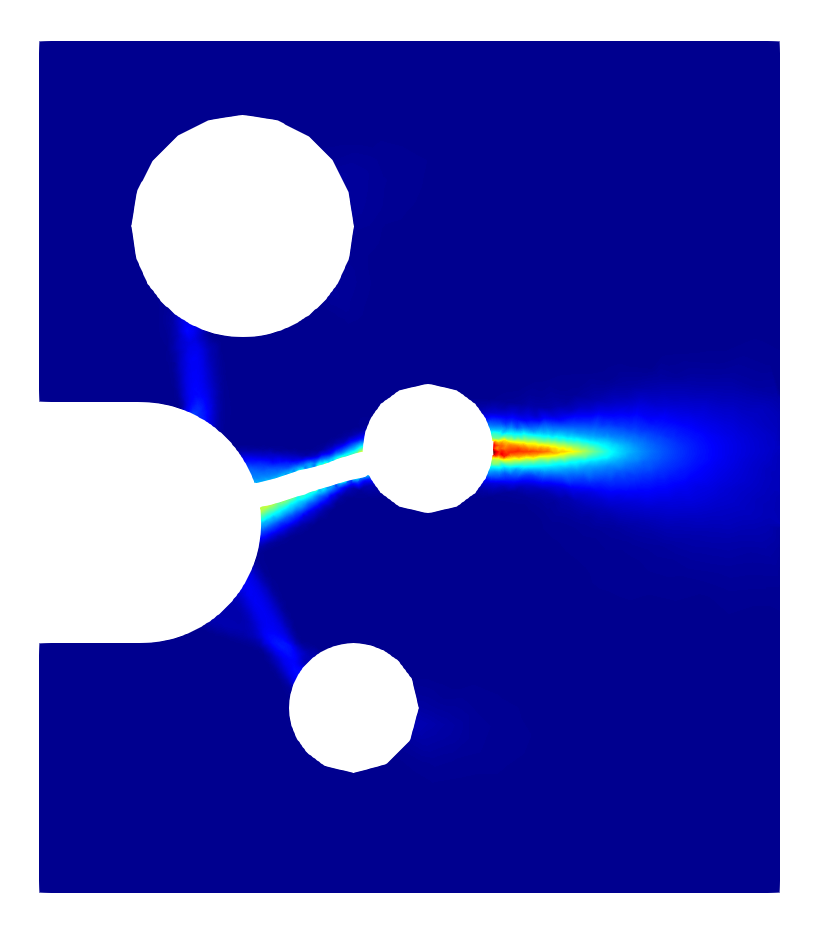
\includegraphics[width=\textwidth,scale=0.5]{Chapter5/figures/SFC/W_pl_2}
    \caption{$u = \SI{5.28}{\milli\meter}$}
    \label{fig: Chapter5/SFC/Wp_2}
  \end{subfigure}
  \hspace{0.03\textwidth}
  \begin{subfigure}{0.2\textwidth}
    \centering
    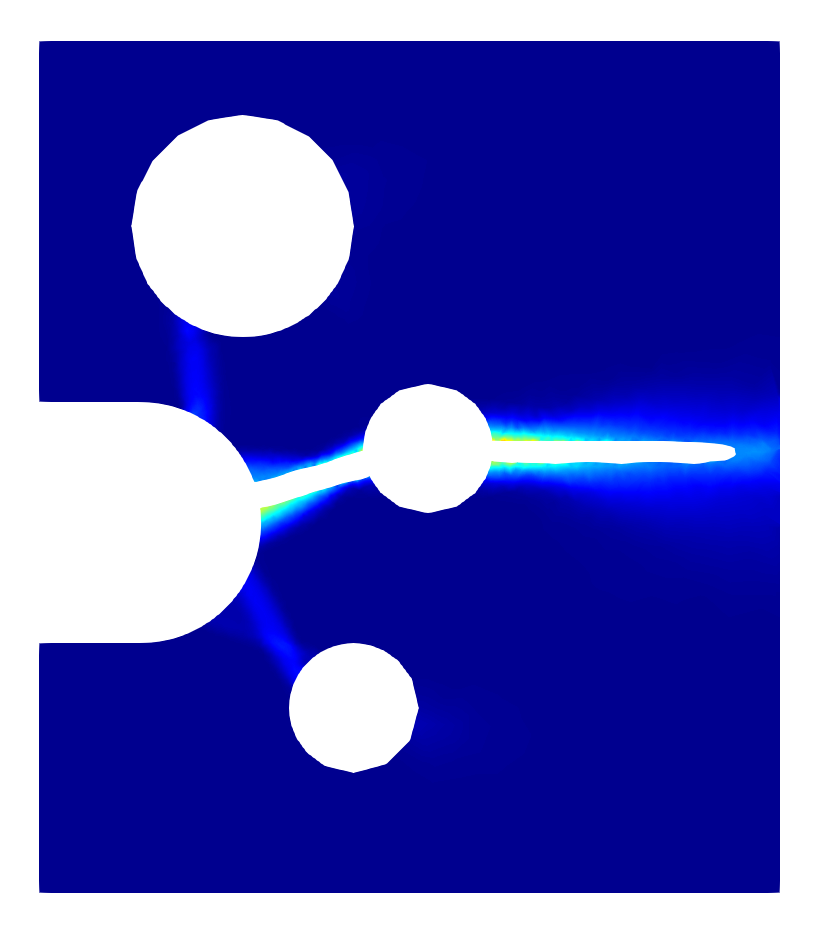
\includegraphics[width=\textwidth,scale=0.5]{Chapter5/figures/SFC/W_pl_3}
    \caption{$u = \SI{6.81}{\milli\meter}$}
    \label{fig: Chapter5/SFC/Wp_3}
  \end{subfigure}
  \begin{subfigure}{0.05\textwidth}
    \centering
    \caption*{$\psi^p$}
    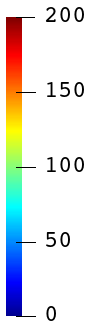
\includegraphics[width=\textwidth,scale=0.5]{Chapter5/figures/SFC/colorbar_Wp_vertical}
    \vspace{1em}
  \end{subfigure}
  
  \begin{subfigure}{0.2\textwidth}
    \centering
    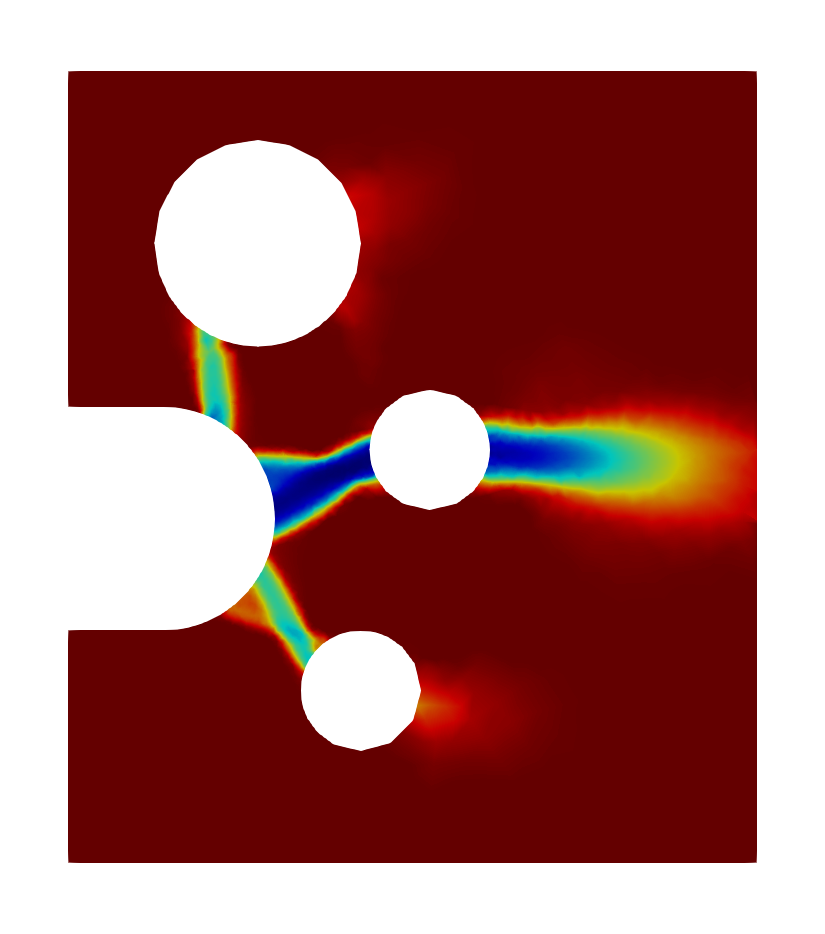
\includegraphics[width=\textwidth,scale=0.5]{Chapter5/figures/SFC/M_1}
    \caption{$u = \SI{2.87}{\milli\meter}$}
    \label{fig: Chapter5/SFC/gc_1}
  \end{subfigure}
  \hspace{0.03\textwidth}
  \begin{subfigure}{0.2\textwidth}
    \centering
    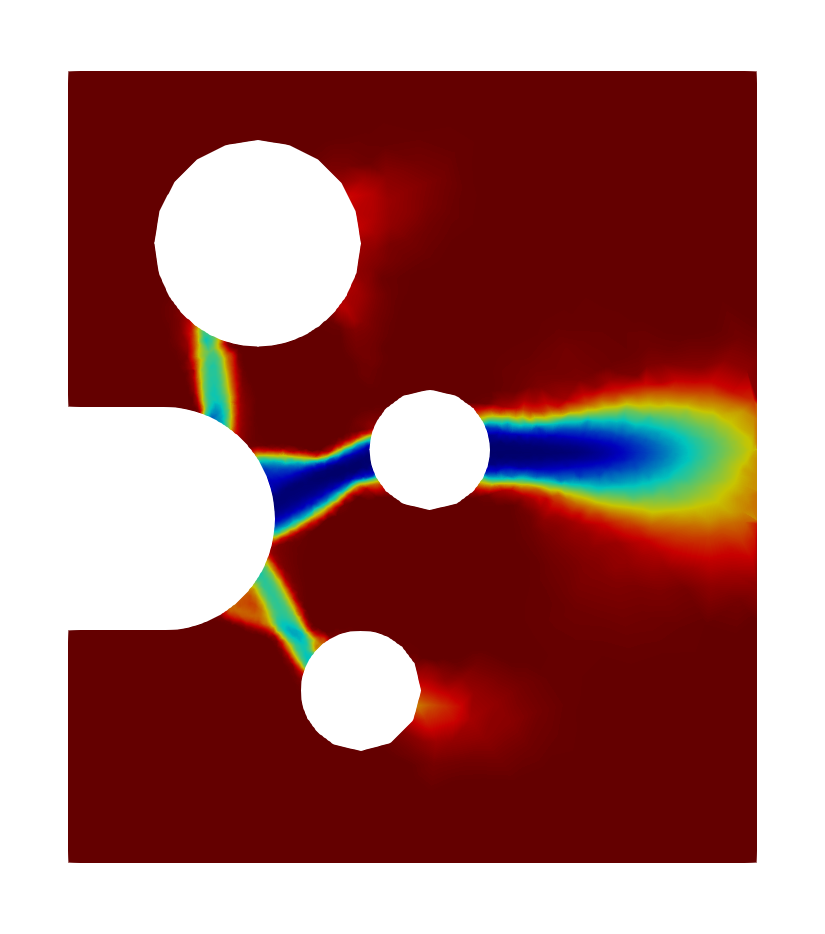
\includegraphics[width=\textwidth,scale=0.5]{Chapter5/figures/SFC/M_2}
    \caption{$u = \SI{5.28}{\milli\meter}$}
    \label{fig: Chapter5/SFC/gc_2}
  \end{subfigure}
  \hspace{0.03\textwidth}
  \begin{subfigure}{0.2\textwidth}
    \centering
    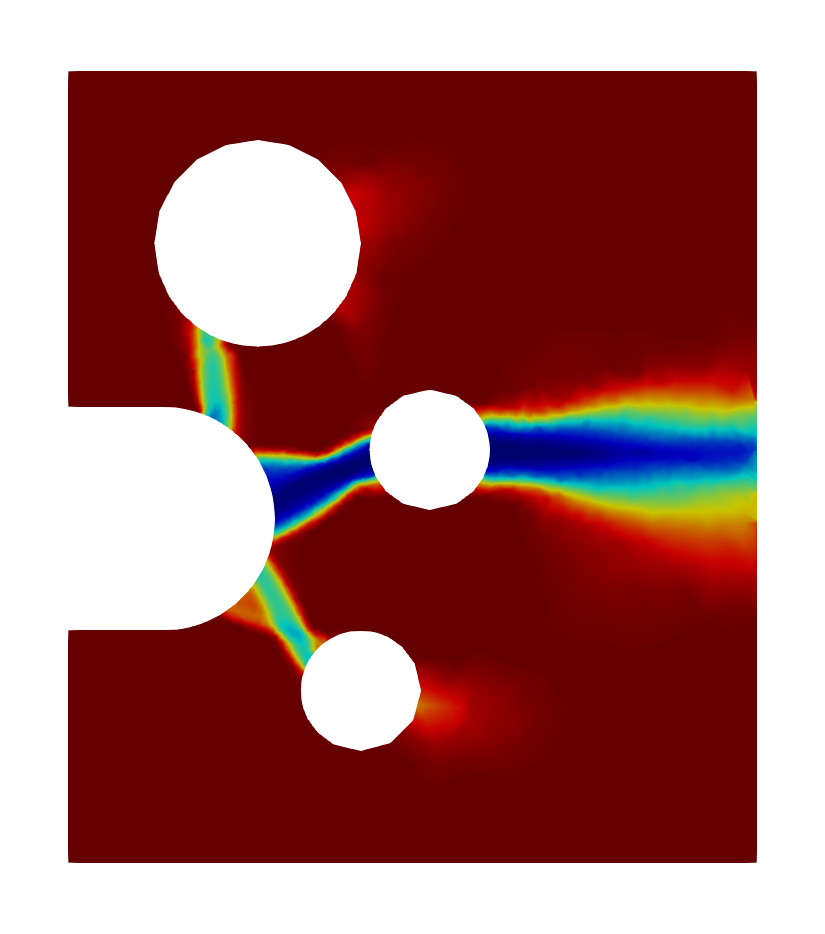
\includegraphics[width=\textwidth,scale=0.5]{Chapter5/figures/SFC/M_3}
    \caption{$u = \SI{6.81}{\milli\meter}$}
    \label{fig: Chapter5/SFC/gc_3}
  \end{subfigure}
  \begin{subfigure}{0.05\textwidth}
    \centering
    \caption*{$g^c$}
    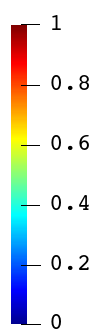
\includegraphics[width=\textwidth,scale=0.5]{Chapter5/figures/SFC/colorbar_gc_vertical}
    \vspace{1em}
  \end{subfigure}
  \caption[Simulation results for the Sandia Fracture Challenge.]{The Sandia Fracture Challenge. Contour plots of (a-c) the phase field $d$, (d-f) the active part of the strain energy $\psi^e_\activepart$, (g-i) the plastic energy $\psi^p$, and (j-l) the coalescence degradation function $g^c$ at three different loads. In subfigures (d-i) the domain within the contour of $d>0.8$ is removed to facilitate crack path visualization. }
\end{figure}



%%%%%%%%%%%%%%%%%%%%%%%%%%%%%%%%%%%%%%%%%%%%%%%%%%%%%%%%%%%%%%%%%%%%%%%%%%%%%%%%%%%%%%%%%%%
%%%%%%%%%%%%%%%%%%%%%%%%%%%%%%%%%%%%%%%%%%%%%%%%%%%%%%%%%%%%%%%%%%%%%%%%%%%%%%%%%%%%%%%%%%%
%%%%%%%%%%%%%%%%%%%%%%%%%%%%%%%%%%%%%%%%%%%%%%%%%%%%%%%%%%%%%%%%%%%%%%%%%%%%%%%%%%%%%%%%%%%
%%%%%%%%%%%%%%%%%%%%%%%%%%%%%%%%%%%%%%%%%%%%%%%%%%%%%%%%%%%%%%%%%%%%%%%%%%%%%%%%%%%%%%%%%%%
%%%%%%%%%%%%%%%%%%%%%%%%%%%%%%%%%%%%%%%%%%%%%%%%%%%%%%%%%%%%%%%%%%%%%%%%%%%%%%%%%%%%%%%%%%%
%%%%%%%%%%%%%%%%%%%%%%%%%%%%%%%%%%%%%%%%%%%%%%%%%%%%%%%%%%%%%%%%%%%%%%%%%%%%%%%%%%%%%%%%%%%
%%%%%%%%%%%%%%%%%%%%%%%%%%%%%%%%%%%%%%%%%%%%%%%%%%%%%%%%%%%%%%%%%%%%%%%%%%%%%%%%%%%%%%%%%%%
%%%%%%%%%%%%%%%%%%%%%%%%%%%%%%%%%%%%%%%%%%%%%%%%%%%%%%%%%%%%%%%%%%%%%%%%%%%%%%%%%%%%%%%%%%%
%%%%%%%%%%%%%%%%%%%%%%%%%%%%%%%%%%%%%%%%%%%%%%%%%%%%%%%%%%%%%%%%%%%%%%%%%%%%%%%%%%%%%%%%%%%
%%%%%%%%%%%%%%%%%%%%%%%%%%%%%%%%%%%%%%%%%%%%%%%%%%%%%%%%%%%%%%%%%%%%%%%%%%%%%%%%%%%%%%%%%%%
\subsection{Spallation of oxidation scale}
\label{section: Chapter5/examples/spallation}

Next, we extend the ductile fracture model within the variational framework to construct a coupled thermo-elasto-creep model to simulate the spallation of oxide scale on high temperature heat exchangers.

High temperature heat exchangers (HTHXs) are key components of many power conversion systems, including advanced nuclear power generation systems. HTHXs typically operate in the inlet temperature range of 750-1100 \SI{}{\celsius} and are subject to unique operating challenges including oxidation, corrosion, creep and fracture.  We focus on modeling the mechanical response of the metal operating at high temperatures, with the objective of developing physics-based models for predicting fracture and spallation of the scale, which will provide insight into the lifetime performance of the heat exchanger.

\begin{figure}
  \centering
  \begin{subfigure}{0.4\textwidth}
    \centering
    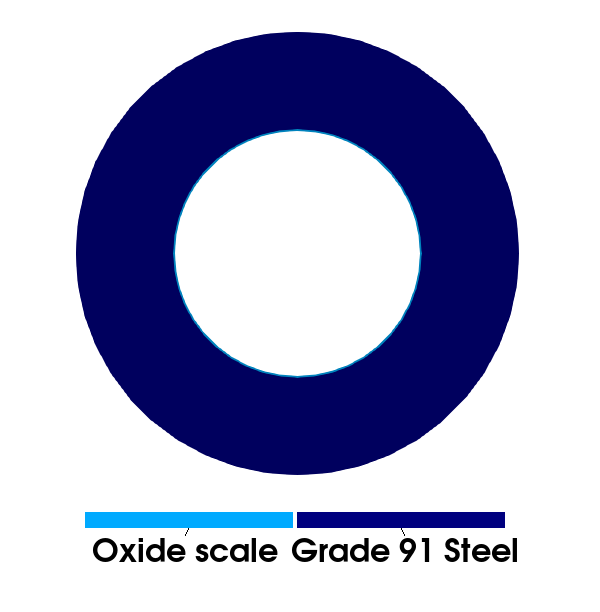
\includegraphics[width=\textwidth]{Chapter5/figures/spallation/top_view}
    \caption{}
  \end{subfigure}
  \begin{subfigure}{0.4\textwidth}
    \centering
    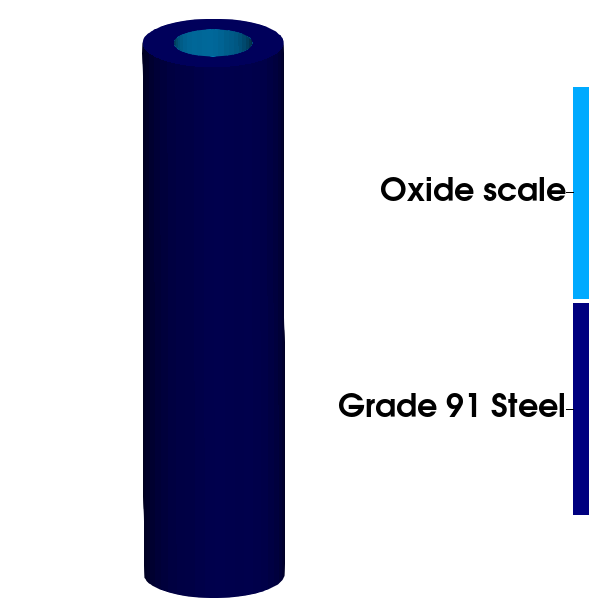
\includegraphics[width=\textwidth]{Chapter5/figures/spallation/side_view}
    \caption{}
  \end{subfigure}
  \caption[Schematics of the heat exchanger.]{(a) Top view and (b) side view of the section of the heat exchanger.}
  \label{fig: Chapter5/spallation/schematics}
\end{figure}


Consider a \SI{30}{\milli\meter}-long section of a metal tube with inner radius \SI{14}{\milli\meter} and outer radius \SI{25}{\milli\meter} (\Cref{fig: Chapter5/spallation/schematics}). Steam flows through the tube, and the tube is surrounded by flue gas. Both the steam and the flue gas are assumed to have a homogeneous temperature and pressure within the control volume at a given instant. The oxide growth on the inner surface of the metal tube is of particular interest. In this section, oxide is assumed to grow following the relation
\begin{align}
  \tau = \sqrt{2A_\text{ox}\exp\left( -\dfrac{Q_\text{ox}}{RT} \right) t},
\end{align}
where $\tau$ is the thickness of the oxide layer, $A_\text{ox}$ is the growth coefficient, $Q_\text{ox}$ is the oxidation activation energy, $R$ is the ideal gas constant, and $T$ is the temperature on the inner surface of the tube.

%%%%%%%%%%%%%%%%%%%%%%%%%%%%%%%%%%%%%%%%%%%%%%%%%%%%%%%%%%%%%%%%%%%%%%%%%%%%%%%%%%%%%%%%%%%
%%%%%%%%%%%%%%%%%%%%%%%%%%%%%%%%%%%%%%%%%%%%%%%%%%%%%%%%%%%%%%%%%%%%%%%%%%%%%%%%%%%%%%%%%%%
%%%%%%%%%%%%%%%%%%%%%%%%%%%%%%%%%%%%%%%%%%%%%%%%%%%%%%%%%%%%%%%%%%%%%%%%%%%%%%%%%%%%%%%%%%%
%%%%%%%%%%%%%%%%%%%%%%%%%%%%%%%%%%%%%%%%%%%%%%%%%%%%%%%%%%%%%%%%%%%%%%%%%%%%%%%%%%%%%%%%%%%
%%%%%%%%%%%%%%%%%%%%%%%%%%%%%%%%%%%%%%%%%%%%%%%%%%%%%%%%%%%%%%%%%%%%%%%%%%%%%%%%%%%%%%%%%%%
%%%%%%%%%%%%%%%%%%%%%%%%%%%%%%%%%%%%%%%%%%%%%%%%%%%%%%%%%%%%%%%%%%%%%%%%%%%%%%%%%%%%%%%%%%%
%%%%%%%%%%%%%%%%%%%%%%%%%%%%%%%%%%%%%%%%%%%%%%%%%%%%%%%%%%%%%%%%%%%%%%%%%%%%%%%%%%%%%%%%%%%
%%%%%%%%%%%%%%%%%%%%%%%%%%%%%%%%%%%%%%%%%%%%%%%%%%%%%%%%%%%%%%%%%%%%%%%%%%%%%%%%%%%%%%%%%%%
%%%%%%%%%%%%%%%%%%%%%%%%%%%%%%%%%%%%%%%%%%%%%%%%%%%%%%%%%%%%%%%%%%%%%%%%%%%%%%%%%%%%%%%%%%%
%%%%%%%%%%%%%%%%%%%%%%%%%%%%%%%%%%%%%%%%%%%%%%%%%%%%%%%%%%%%%%%%%%%%%%%%%%%%%%%%%%%%%%%%%%%
\subsubsection{Incorporating debonding}

The power-law creep model presented in \Cref{section: Chapter5/theory} is used to model the mechanical response of the metal. In particular, the creep response is assumed to be quasi-static, therefore no viscous effects are incorporated, i.e. ${\psi^e}^* = {\psi^p}^* = {\psi^f}^* = 0$. It is assumed that the metal does not fracture during the spallation process, therefore $\psi^f = 0$ in the metal. The interface between the oxide and the metal is modeled together with the oxide layer, and they are represented as a lower-dimensional manifold attached on the inner surface of the metal tube. Under the assumption that the thickness of the oxide is much smaller than that of the metal tube, both in-plane transverse cracks and out-of-plane debonding at the oxide-metal interface could be represented on the same manifold, with proper enrichment to the constitutive model.

The modified fracture energy density of the oxide is extended to consider debonding at the oxide-metal interface. Debonding at the interface is associated with the release of energy, i.e. $\int\limits_D \mathcal{G} \diff{A}$, where $D$ is the debonded region, and $\mathcal{G}$ is the energy release rate per unit debonded area. Under the assumption that the oxide layer is sufficiently thin, the interface energy can be smeared by an auxiliary field $c$ and uniformly distributed throughout the thickness of the oxide, i.e.
\begin{align}
  \psi^f = \dfrac{\Gc}{c_0 l} \left( C\alpha(d) + l^2 \grad d \cdot \grad d \right) + \dfrac{1}{\tau} \mathcal{G} \omega(c),
\end{align}
where $\omega(c)$ is the characteristic function for the debonding area, and $\omega(0) = 0$, $\omega(1) = 1$.

The strain energy density of the oxide is defined in the local coordinate system attached to each material point. The global coordinate system is transformed such that the local $z$-axis aligns with the exterior normal of the oxide. The transformation tensor $\bfT$ is computed using the Rodrigues formula:
\begin{align}
  T_{ij}(\hat{\normal}, \theta) = \cos(\theta)\delta_{ij} + \left[ 1-\cos(\theta) \right] n_in_j + \sin(\theta)\epsilon_{ijk}n_k,
\end{align}
where $\hat{\normal}$ is the axis of rotation, $\theta$ is the rotation angle, and $\bs{\epsilon}$ is the permutation tensor. The Hencky-type logarithmic strain measure is used for the oxide. The strain is first transformed into the local coordinate system by ${\strain^e}' = \bfT {\strain^e} \bfT^T$ and decomposed into in-plane and out-of-plane components
\begin{subequations}
  \begin{align}
    {\strain^e_\text{ip}}' & = \bfE_\text{ip} {\strain^e}' \bfE_\text{ip}^T,                      \\
    {\strain^e_\text{op}}' & = \strain' - \bfE_\text{ip}^T {\strain^e_\text{ip}}' \bfE_\text{ip}, 
  \end{align}
\end{subequations}
where $\bfE_\text{ip}$ is the embedding matrix for the in-plane components, defined as
\begin{align}
  \bfE_\text{ip} =
  \begin{bmatrix}
    1 & 0 & 0 \\
    0 & 1 & 0 
  \end{bmatrix}.
\end{align}
The modified strain energy density is then defined as
\begin{subequations}
  \begin{align}
    \psi^e                            & =  g^e_\text{ip} \psi^e_{\text{ip}, \activepart} + \psi^e_{\text{ip}, \inactivepart} + g^e_\text{op} \psi^e_{\text{op}, \activepart} + \psi^e_{\text{ip}, \inactivepart},                                                                           \\
    \psi^e_{\text{ip}, \activepart}   & = \dfrac{1}{2} K \macaulay{\tr({\strain^e_\text{ip}}')}_+^2 + G \dev{{\strain^e_\text{ip}}'} : \dev{{\strain^e_\text{ip}}'},                                                                                                                        \\
    \psi^e_{\text{ip}, \inactivepart} & = \dfrac{1}{2} K \macaulay{\tr({\strain^e_\text{ip}}')}_-^2,                                                                                                                                                                                        \\
    \psi^e_{\text{op}, \activepart}   & = \dfrac{1}{2} K \macaulay{{\varepsilon^e_\text{op}}'}_+^2 + G \left( {\strain^e_\text{op}}' - {\varepsilon^e_\text{op}}' \bte_3 \otimes \bte_3 \right) : \left( {\strain^e_\text{op}}' - {\varepsilon^e_\text{op}}' \bte_3 \otimes \bte_3 \right), \\
    \psi^e_{\text{op}, \inactivepart} & = \dfrac{1}{2} K \macaulay{{\varepsilon^e_\text{op}}'}_-^2.,                                                                                                                                                                                        \\
    {\varepsilon^e_\text{op}}'        & = \bte_3 \cdot {\strain^e_\text{op}}' \bte_3,                                                                                                                                                                                                       
  \end{align}
\end{subequations}
where $g^e_\text{ip}$ and $g^e_\text{op}$ are the in-plane and the out-of-plane degradation functions, respectively.

The modified Piola stress $\bfP^\text{eq}$ follow from the constitutive restrictions \eqref{eq: constitutive restrictions}. Furthermore, minimizing with respect to $c$ (together with the irreversibility condition $\dot{c} \geqslant 0$) leads to the following KKT conditions:
\begin{align}
  \phi^i = - \dfrac{1}{\tau} \mathcal{G} \omega_{,c} - \psi^e_{,c} \leqslant 0, \quad \dot{c} \geqslant 0, \quad \phi^i \dot{c} = 0.
\end{align}

The following constitutive functions are chosen in this section, such that both the in-plane transverse fracture and the out-of-plane debonding are characterized by a linear traction-separation law:
\begin{subequations}
  \begin{align}
     & \alpha = d, \quad \omega = c, \quad g^p = 1,                                                           \\
     & g^e = g^e_\text{ip} = \dfrac{(1-d)^2}{(1-d)^2 + m_\text{ip} d (1 - 0.5 d)},                            \\
     & g^e_\text{op} = \dfrac{(1-c)^2}{(1-c)^2 + m_\text{op} c (1 - 0.5 c)},                                  \\
     & m_\text{ip} = \dfrac{3}{8l}\dfrac{\Gc}{\psi_c}, \quad m_\text{op} = \dfrac{\mathcal{G}}{\tau\psi^i_c}, 
  \end{align}
\end{subequations}
where $\psi_c$ is the in-plane critical fracture energy density, and $\psi^i_c$ is the out-of-plane critical fracture energy density.

%%%%%%%%%%%%%%%%%%%%%%%%%%%%%%%%%%%%%%%%%%%%%%%%%%%%%%%%%%%%%%%%%%%%%%%%%%%%%%%%%%%%%%%%%%%
%%%%%%%%%%%%%%%%%%%%%%%%%%%%%%%%%%%%%%%%%%%%%%%%%%%%%%%%%%%%%%%%%%%%%%%%%%%%%%%%%%%%%%%%%%%
%%%%%%%%%%%%%%%%%%%%%%%%%%%%%%%%%%%%%%%%%%%%%%%%%%%%%%%%%%%%%%%%%%%%%%%%%%%%%%%%%%%%%%%%%%%
%%%%%%%%%%%%%%%%%%%%%%%%%%%%%%%%%%%%%%%%%%%%%%%%%%%%%%%%%%%%%%%%%%%%%%%%%%%%%%%%%%%%%%%%%%%
%%%%%%%%%%%%%%%%%%%%%%%%%%%%%%%%%%%%%%%%%%%%%%%%%%%%%%%%%%%%%%%%%%%%%%%%%%%%%%%%%%%%%%%%%%%
%%%%%%%%%%%%%%%%%%%%%%%%%%%%%%%%%%%%%%%%%%%%%%%%%%%%%%%%%%%%%%%%%%%%%%%%%%%%%%%%%%%%%%%%%%%
%%%%%%%%%%%%%%%%%%%%%%%%%%%%%%%%%%%%%%%%%%%%%%%%%%%%%%%%%%%%%%%%%%%%%%%%%%%%%%%%%%%%%%%%%%%
%%%%%%%%%%%%%%%%%%%%%%%%%%%%%%%%%%%%%%%%%%%%%%%%%%%%%%%%%%%%%%%%%%%%%%%%%%%%%%%%%%%%%%%%%%%
%%%%%%%%%%%%%%%%%%%%%%%%%%%%%%%%%%%%%%%%%%%%%%%%%%%%%%%%%%%%%%%%%%%%%%%%%%%%%%%%%%%%%%%%%%%
%%%%%%%%%%%%%%%%%%%%%%%%%%%%%%%%%%%%%%%%%%%%%%%%%%%%%%%%%%%%%%%%%%%%%%%%%%%%%%%%%%%%%%%%%%%
\subsubsection{Boundary conditions}

For convenience, boundaries of the section of the heat exchanger under consideration are marked in \Cref{fig: Chapter5/spallation/boundaries}. Utilizing symmetry, only a quarter of the domain is modeled. Symmetry conditions, i.e. $\btu \cdot \normal_0 = 0$ and $\grad T \cdot \normal_0 = 0$, are enforced on the sides. The bottom of the section is fixed in the $z$-direction, i.e. $u_z = 0$. The inner and outer surfaces are subjected to pressure and heat convection.
The Pressure and temperature of the steam and the flue gas are summarized in \Cref{table: Chapter5/spallation/schedule} for different operating conditions. The operation of the heat exchanger cycles between the full and the partial schedule. The heat exchanger shuts down after 6 months of normal operation, during which the temperature of the steam and the flue gas drops to the room temperature, and the pressure becomes negligible. Since the actual heat exchanger is longer than the section under consideration, generalized plane strain conditions are assumed to hold on the top surface of the tube, i.e. $\int\limits_{\bodyboundary_0} \normal_0 \cdot \strain \normal_0 \diff{A} = 0 $.

\begin{figure}[!htb]
  \centering
  \begin{subfigure}{0.19\textwidth}
    \centering
    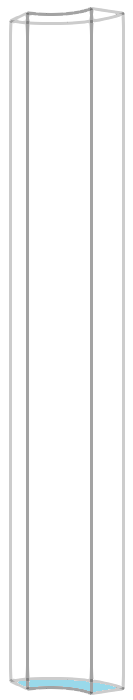
\includegraphics[width=0.6\textwidth]{Chapter5/figures/spallation/geometry_bottom}
    \caption{Bottom}
  \end{subfigure}
  \begin{subfigure}{0.19\textwidth}
    \centering
    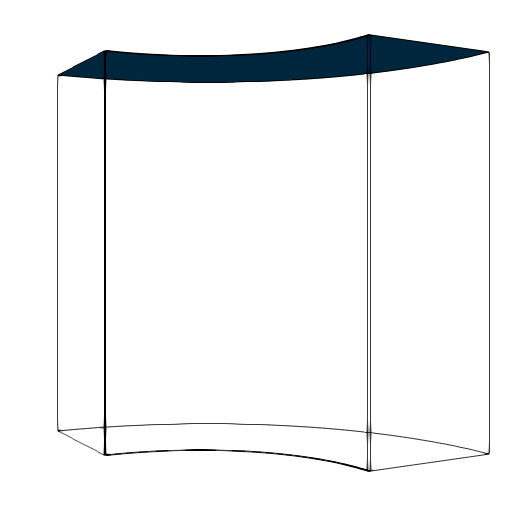
\includegraphics[width=0.6\textwidth]{Chapter5/figures/spallation/geometry_top}
    \caption{Top}
  \end{subfigure}
  \begin{subfigure}{0.19\textwidth}
    \centering
    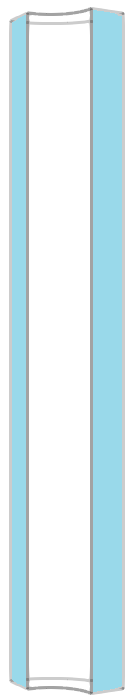
\includegraphics[width=0.6\textwidth]{Chapter5/figures/spallation/geometry_sides}
    \caption{Sides}
  \end{subfigure}
  \begin{subfigure}{0.19\textwidth}
    \centering
    \includegraphics[width=0.6\textwidth]{Chapter5/figures/spallation/geometry_inner}
    \caption{Inner surface}
  \end{subfigure}
  \begin{subfigure}{0.19\textwidth}
    \centering
    \includegraphics[width=0.6\textwidth]{Chapter5/figures/spallation/geometry_outer}
    \caption{Outer surface}
  \end{subfigure}
  \caption{Boundaries of the heat exchanger.}
  \label{fig: Chapter5/spallation/boundaries}
\end{figure}


\begin{table}[!htb]
  \small
  \centering
  \caption{Summary of operation schedule}
  \label{table: Chapter5/spallation/schedule}
  \begin{tabular}{r c c c c c c}
    \toprule
    Load     & Duration (\SI{}{\hour}) & $T_s$ (\SI{}{\celsius}) & $T_g$ (\SI{}{\celsius}) & $p_s$ (\SI{}{\mega\pascal}) & $p_g$ (\SI{}{\mega\pascal}) & Transition (\SI{}{\hour}) \\
    \midrule
    Full     & 14                      & 530                     & 1100                    & 17                          & 0.2                         & Full to Partial: 1        \\
    Partial  & 8                       & 525                     & 845                     & 10                          & 0.1                         & Partial to Full: 1        \\
    Shutdown & 25                      & 25                      & 25                      & 0.1                         & 0.1                         & Full to Shutdown: 6       \\
    \bottomrule
  \end{tabular}
\end{table}

%%%%%%%%%%%%%%%%%%%%%%%%%%%%%%%%%%%%%%%%%%%%%%%%%%%%%%%%%%%%%%%%%%%%%%%%%%%%%%%%%%%%%%%%%%%
%%%%%%%%%%%%%%%%%%%%%%%%%%%%%%%%%%%%%%%%%%%%%%%%%%%%%%%%%%%%%%%%%%%%%%%%%%%%%%%%%%%%%%%%%%%
%%%%%%%%%%%%%%%%%%%%%%%%%%%%%%%%%%%%%%%%%%%%%%%%%%%%%%%%%%%%%%%%%%%%%%%%%%%%%%%%%%%%%%%%%%%
%%%%%%%%%%%%%%%%%%%%%%%%%%%%%%%%%%%%%%%%%%%%%%%%%%%%%%%%%%%%%%%%%%%%%%%%%%%%%%%%%%%%%%%%%%%
%%%%%%%%%%%%%%%%%%%%%%%%%%%%%%%%%%%%%%%%%%%%%%%%%%%%%%%%%%%%%%%%%%%%%%%%%%%%%%%%%%%%%%%%%%%
%%%%%%%%%%%%%%%%%%%%%%%%%%%%%%%%%%%%%%%%%%%%%%%%%%%%%%%%%%%%%%%%%%%%%%%%%%%%%%%%%%%%%%%%%%%
%%%%%%%%%%%%%%%%%%%%%%%%%%%%%%%%%%%%%%%%%%%%%%%%%%%%%%%%%%%%%%%%%%%%%%%%%%%%%%%%%%%%%%%%%%%
%%%%%%%%%%%%%%%%%%%%%%%%%%%%%%%%%%%%%%%%%%%%%%%%%%%%%%%%%%%%%%%%%%%%%%%%%%%%%%%%%%%%%%%%%%%
%%%%%%%%%%%%%%%%%%%%%%%%%%%%%%%%%%%%%%%%%%%%%%%%%%%%%%%%%%%%%%%%%%%%%%%%%%%%%%%%%%%%%%%%%%%
%%%%%%%%%%%%%%%%%%%%%%%%%%%%%%%%%%%%%%%%%%%%%%%%%%%%%%%%%%%%%%%%%%%%%%%%%%%%%%%%%%%%%%%%%%%
\subsubsection{Model parameters and material properties}

Model parameters and material properties for the oxide and the metal are summarized in \Cref{table: Chapter5/spallation/oxide,table: Chapter5/spallation/metal}, respectively. Most material properties are taken in accordance with \cite{xue2020stress} for comparison purposes.
Following \Cref{remark: tqf}, since the creep activation energy for both the oxide and the metal are much larger than the product of the ideal gas constant and the temperature, i.e. $Q \gg RT$, we take $\tqf = 1$ to satisfy the second law of thermodynamics. The fracture toughness $\Gc$ of the oxide layer is taken in the ballpark of that of Cr$_2$O$_3$. Due to the lack of experimental measurements, both the in-plane and the out-of-plane critical fracture energy density are chosen such that the transverse fracture energy and the debonding energy are of the same order of magnitude during the spallation process. To introduce coupling between plasticity and fracture, the coalescence dissipation (see \Cref{section: Chapter5/theory/constitutive/fracture}) is included with $\beta = 0.3$ and $\varepsilon_0 = \SI{1e-6}{}$.

\begin{table}[!htb]
  \small
  \centering
  \caption{Summary of material properties and model parameters for the oxide}
  \label{table: Chapter5/spallation/oxide}
  \begin{tabular}{r c c c}
    \toprule
    Property/Parameter                            & Symbol          & Value           & Unit                                       \\
    \midrule
    Young's modulus                               & $E$             & 120             & \SI{}{\giga\pascal}                        \\
    Poisson's ratio                               & $\nu$           & 0.24            & nondim.                                    \\
    Thermal conductivity                          & $\kappa$        & 3               & \SI{}{\watt\per\meter\per\kelvin}          \\
    Convection coefficient (steam-oxide)          & $h$             & 2800            & \SI{}{\watt\per\square\meter\per\kelvin}   \\
    Creep coefficient                             & $A$             & \SI{8.5875e7}{} & \SI{}{\per\second}                         \\
    Creep exponent                                & $n$             & \SI{3}{}        & nondim.                                    \\
    Creep activation energy                       & $Q$             & \SI{421.62}{}   & \SI{}{\kilo\joule\per\mole}                \\
    Taylor-Quinney factor                         & $\tqf$          & 1               & nondim.                                    \\
    In-plane fracture toughness                   & $\Gc$           & \SI{0.025}{}    & \SI{}{\milli\joule\per\square\milli\meter} \\
    In-plane critical fracture energy density     & $\psi_c$        & \SI{0.008}{}    & \SI{}{\milli\joule\per\cubic\milli\meter}  \\
    Out-of-plane fracture toughness               & $\mathcal{G}$   & \SI{2.5e-7}{}   & \SI{}{\milli\joule\per\square\milli\meter} \\
    Out-of-plane critical fracture energy density & $\psi_c^i$      & \SI{5e-7}{}     & \SI{}{\milli\joule\per\cubic\milli\meter}  \\
    Regularization length                         & $l$             & \SI{0.25}{}     & \SI{}{\milli\meter}                        \\
    Interaction coefficient                       & $\beta$         & \SI{0.05}{}     & nondim.                                    \\
    Characteristic creep strain                   & $\varepsilon_0$ & \SI{1e-6}{}     & nondim.                                    \\
    Oxidation coefficient                         & $A_\text{ox}$   & \SI{6.22e8}{}   & \SI{}{\square\meter\per\hour}              \\
    Oxidation activation energy                   & $Q_\text{ox}$   & 326             & \SI{}{\kilo\joule\per\mole}                \\
    \bottomrule
  \end{tabular}
\end{table}

\begin{table}[!htb]
  \small
  \centering
  \caption{Summary of material properties and model parameters for the metal}
  \label{table: Chapter5/spallation/metal}
  \begin{tabular}{r c c c}
    \toprule
    Property/Parameter                 & Symbol   & Value        & Unit                                     \\
    \midrule
    Young's modulus                    & $E$      & 190          & \SI{}{\giga\pascal}                      \\
    Poisson's ratio                    & $\nu$    & 0.3          & nondim.                                  \\
    Thermal conductivity               & $\kappa$ & 30           & \SI{}{\watt\per\meter\per\kelvin}        \\
    Convection coefficient (metal-gas) & $h$      & 100          & \SI{}{\watt\per\square\meter\per\kelvin} \\
    Creep coefficient                  & $A$      & \SI{2.3e6}{} & \SI{}{\per\second}                       \\
    Creep exponent                     & $n$      & \SI{5.06}{}  & nondim.                                  \\
    Creep activation energy            & $Q$      & 400          & \SI{}{\kilo\joule\per\mole}              \\
    Taylor-Quinney factor              & $\tqf$   & 1            & nondim.                                  \\
    \bottomrule
  \end{tabular}
\end{table}

The thermal expansion is accounted for by the thermal deformation gradient $\bfF^g$ defined in terms of the measured instantaneous isotropic coefficient of thermal expansion $\bar{\alpha}$:
\begin{align}
  \bfF^g = \left( 1 + \int\limits_{T_0}^T \alpha \diff{T'} \right) \bfI,
\end{align}
where $T_0$ is the reference stress-free temperature. Since the oxide mainly forms at high temperature, the temperature profile obtained with the full operating conditions is considered to be the reference temperature. The instantaneous coefficients of thermal expansion are taken in accordance with \cite{xue2020stress} and are shown in \Cref{fig: Chapter5/spallation/cte}.

\begin{figure}[htb!]
  \centering
  \begin{tikzpicture}
    \begin{axis}[
        colormap/jet,
        cycle list={[of colormap,samples of colormap=2]},
        width=0.6\textwidth,
        height=0.5\textwidth,
        xlabel=Temperature (\SI{}{\celsius}),
        ylabel=$\alpha$,
        scaled x ticks=false,
        yticklabel style={
            /pgf/number format/fixed,
            /pgf/number format/precision=2
          },
        xticklabel style={
            /pgf/number format/fixed,
            /pgf/number format/precision=2
          },
        legend style={
            at={(0.95,0.05)},
            anchor=south east,
            nodes={scale=1.2, transform shape},
            fill=white,
            fill opacity=0.8,
            draw opacity=1,
            text opacity=1,
            cells={align=left}
          },
        legend cell align={left},
        every axis plot/.append style={thick,no marks}
      ]
      \addplot table[x expr=\thisrowno{0},y expr=\thisrowno{1},col sep=comma]{Chapter5/data/spallation/CTE_oxide.csv};
      \addplot table[x expr=\thisrowno{0},y expr=\thisrowno{1},col sep=comma]{Chapter5/data/spallation/CTE_metal.csv};
      \legend{oxide, metal}
    \end{axis}
  \end{tikzpicture}
  \caption{Instantaneous thermal expansion coefficients.}
  \label{fig: Chapter5/spallation/cte}
\end{figure}


%%%%%%%%%%%%%%%%%%%%%%%%%%%%%%%%%%%%%%%%%%%%%%%%%%%%%%%%%%%%%%%%%%%%%%%%%%%%%%%%%%%%%%%%%%%
%%%%%%%%%%%%%%%%%%%%%%%%%%%%%%%%%%%%%%%%%%%%%%%%%%%%%%%%%%%%%%%%%%%%%%%%%%%%%%%%%%%%%%%%%%%
%%%%%%%%%%%%%%%%%%%%%%%%%%%%%%%%%%%%%%%%%%%%%%%%%%%%%%%%%%%%%%%%%%%%%%%%%%%%%%%%%%%%%%%%%%%
%%%%%%%%%%%%%%%%%%%%%%%%%%%%%%%%%%%%%%%%%%%%%%%%%%%%%%%%%%%%%%%%%%%%%%%%%%%%%%%%%%%%%%%%%%%
%%%%%%%%%%%%%%%%%%%%%%%%%%%%%%%%%%%%%%%%%%%%%%%%%%%%%%%%%%%%%%%%%%%%%%%%%%%%%%%%%%%%%%%%%%%
%%%%%%%%%%%%%%%%%%%%%%%%%%%%%%%%%%%%%%%%%%%%%%%%%%%%%%%%%%%%%%%%%%%%%%%%%%%%%%%%%%%%%%%%%%%
%%%%%%%%%%%%%%%%%%%%%%%%%%%%%%%%%%%%%%%%%%%%%%%%%%%%%%%%%%%%%%%%%%%%%%%%%%%%%%%%%%%%%%%%%%%
%%%%%%%%%%%%%%%%%%%%%%%%%%%%%%%%%%%%%%%%%%%%%%%%%%%%%%%%%%%%%%%%%%%%%%%%%%%%%%%%%%%%%%%%%%%
%%%%%%%%%%%%%%%%%%%%%%%%%%%%%%%%%%%%%%%%%%%%%%%%%%%%%%%%%%%%%%%%%%%%%%%%%%%%%%%%%%%%%%%%%%%
%%%%%%%%%%%%%%%%%%%%%%%%%%%%%%%%%%%%%%%%%%%%%%%%%%%%%%%%%%%%%%%%%%%%%%%%%%%%%%%%%%%%%%%%%%%
\subsubsection{Debonding around pre-existing cracks}
\label{section: Chapter5/examples/spallation/preexisting}

The model for spallation is first verified by simulating debonding around two pre-existing cracks. Under normal operating conditions at high temperature, the oxide layer is expected to grow thicker and creep, and debonding is expected to occur in the vicinity of the crack surface.
Two small pre-existing cracks are introduced as the initial condition of the phase-field. The crack set is defined by $\Gamma = \{ \btX \ \vert\ \frac{\pi}{6} \leqslant \theta \leqslant \frac{\pi}{3}, \quad \text{X}_3 \in \{ \SI{7.5}{\milli\meter}, \SI{22.5}{\milli\meter} \} \}$, where $\theta = \atan\left( \frac{\text{X}_2}{\text{X}_1} \right)$.
All nodes within the crack set are initialized to have $d = 1$. The debonding indicator is initialized to $c = 0$ everywhere.
The response of the heat exchanger is simulated for 180 days under normal operating conditions followed by a shutdown.
Boundary conditions are generated following the operation schedule indicated in \Cref{table: Chapter5/spallation/schedule}.
The evolution of the phase field $d$, the debonding indicator $c$, and the effective creep strain $\ep$ are shown in \Cref{fig: Chapter5/spallation/animation_seed,fig: Chapter5/spallation/animation_seed_2}.

\begin{figure}[!htb]
  \centering
  \begin{subfigure}[b]{0.2\textwidth}
    \centering
    \includegraphics[width=\textwidth]{Chapter5/figures/spallation/seed_d_1}
    \caption{0 day}
  \end{subfigure}
  \begin{subfigure}[b]{0.2\textwidth}
    \centering
    \includegraphics[width=\textwidth]{Chapter5/figures/spallation/seed_d_2}
    \caption{60 days}
  \end{subfigure}
  \begin{subfigure}[b]{0.2\textwidth}
    \centering
    \includegraphics[width=\textwidth]{Chapter5/figures/spallation/seed_d_3}
    \caption{120 days}
  \end{subfigure}
  \begin{subfigure}[b]{0.2\textwidth}
    \centering
    \includegraphics[width=\textwidth]{Chapter5/figures/spallation/seed_d_4}
    \caption{180 days}
  \end{subfigure}
  \begin{subfigure}[b]{0.1\textwidth}
    \centering
    \caption*{$d$}
    \includegraphics[width=0.6\textwidth]{Chapter5/figures/spallation/colorbar_d_seed}
    \vspace{4em}
  \end{subfigure}
  
  \begin{subfigure}[b]{0.2\textwidth}
    \centering
    \includegraphics[width=\textwidth]{Chapter5/figures/spallation/seed_c_1}
    \caption{0 day}
  \end{subfigure}
  \begin{subfigure}[b]{0.2\textwidth}
    \centering
    \includegraphics[width=\textwidth]{Chapter5/figures/spallation/seed_c_2}
    \caption{60 days}
  \end{subfigure}
  \begin{subfigure}[b]{0.2\textwidth}
    \centering
    \includegraphics[width=\textwidth]{Chapter5/figures/spallation/seed_c_3}
    \caption{120 days}
  \end{subfigure}
  \begin{subfigure}[b]{0.2\textwidth}
    \centering
    \includegraphics[width=\textwidth]{Chapter5/figures/spallation/seed_c_4}
    \caption{180 days}
  \end{subfigure}
  \begin{subfigure}[b]{0.1\textwidth}
    \centering
    \caption*{$c$}
    \includegraphics[width=0.6\textwidth]{Chapter5/figures/spallation/colorbar_c_seed}
    \vspace{4em}
  \end{subfigure}
  
  \begin{subfigure}[b]{0.2\textwidth}
    \centering
    \includegraphics[width=\textwidth]{Chapter5/figures/spallation/seed_ep_1}
    \caption{0 day}
  \end{subfigure}
  \begin{subfigure}[b]{0.2\textwidth}
    \centering
    \includegraphics[width=\textwidth]{Chapter5/figures/spallation/seed_ep_2}
    \caption{60 days}
  \end{subfigure}
  \begin{subfigure}[b]{0.2\textwidth}
    \centering
    \includegraphics[width=\textwidth]{Chapter5/figures/spallation/seed_ep_3}
    \caption{120 days}
  \end{subfigure}
  \begin{subfigure}[b]{0.2\textwidth}
    \centering
    \includegraphics[width=\textwidth]{Chapter5/figures/spallation/seed_ep_4}
    \caption{180 days}
  \end{subfigure}
  \begin{subfigure}[b]{0.1\textwidth}
    \centering
    \caption*{$\ep$}
    \includegraphics[width=0.6\textwidth]{Chapter5/figures/spallation/colorbar_ep_seed}
    \vspace{4em}
  \end{subfigure}
  \caption[Simulation of spallation with a pre-existing crack under normal operating conditions.]{Contour plots of (a-d) the phase field, (e-h) the debonding indicator, and (i-l) the effective creep strain. In the contour plots of the debonding indicator and the effective creep strain, elements within the contour of $d \leqslant 0.75$ are removed to visualize the pre-existing crack. In all contour plots, the oxide layer is warped according to the debonding indicator $c$ to visualize debonding. }
  \label{fig: Chapter5/spallation/animation_seed}
\end{figure}


Under normal operating conditions, temperature in the oxide layer remains high. Creep deformation accumulates. The effective creep strain localizes around the crack tips along their horizontal extensions. Debonding first occurs in the vicinity of the crack tips due to localization of the out-of-plane strain energy, followed by the debonding of a continuous region around the crack.

\begin{figure}[!htb]
  \centering
  \begin{subfigure}[b]{0.2\textwidth}
    \centering
    \includegraphics[width=\textwidth]{Chapter5/figures/spallation/seed_d_4}
    \caption{0 hour}
  \end{subfigure}
  \begin{subfigure}[b]{0.2\textwidth}
    \centering
    \includegraphics[width=\textwidth]{Chapter5/figures/spallation/seed_d_5}
    \caption{1 hour}
  \end{subfigure}
  \begin{subfigure}[b]{0.2\textwidth}
    \centering
    \includegraphics[width=\textwidth]{Chapter5/figures/spallation/seed_d_6}
    \caption{2 hours}
  \end{subfigure}
  \begin{subfigure}[b]{0.2\textwidth}
    \centering
    \includegraphics[width=\textwidth]{Chapter5/figures/spallation/seed_d_7}
    \caption{3 hours}
  \end{subfigure}
  \begin{subfigure}[b]{0.1\textwidth}
    \centering
    \caption*{$d$}
    \includegraphics[width=0.6\textwidth]{Chapter5/figures/spallation/colorbar_d_seed}
    \vspace{4em}
  \end{subfigure}
  
  \begin{subfigure}[b]{0.2\textwidth}
    \centering
    \includegraphics[width=\textwidth]{Chapter5/figures/spallation/seed_c_4}
    \caption{0 hour}
  \end{subfigure}
  \begin{subfigure}[b]{0.2\textwidth}
    \centering
    \includegraphics[width=\textwidth]{Chapter5/figures/spallation/seed_c_5}
    \caption{1 hour}
  \end{subfigure}
  \begin{subfigure}[b]{0.2\textwidth}
    \centering
    \includegraphics[width=\textwidth]{Chapter5/figures/spallation/seed_c_6}
    \caption{2 hours}
  \end{subfigure}
  \begin{subfigure}[b]{0.2\textwidth}
    \centering
    \includegraphics[width=\textwidth]{Chapter5/figures/spallation/seed_c_7}
    \caption{3 hours}
  \end{subfigure}
  \begin{subfigure}[b]{0.1\textwidth}
    \centering
    \caption*{$c$}
    \includegraphics[width=0.6\textwidth]{Chapter5/figures/spallation/colorbar_c_seed}
    \vspace{4em}
  \end{subfigure}
  
  \begin{subfigure}[b]{0.2\textwidth}
    \centering
    \includegraphics[width=\textwidth]{Chapter5/figures/spallation/seed_ep_4}
    \caption{0 hour}
  \end{subfigure}
  \begin{subfigure}[b]{0.2\textwidth}
    \centering
    \includegraphics[width=\textwidth]{Chapter5/figures/spallation/seed_ep_5}
    \caption{1 hour}
  \end{subfigure}
  \begin{subfigure}[b]{0.2\textwidth}
    \centering
    \includegraphics[width=\textwidth]{Chapter5/figures/spallation/seed_ep_6}
    \caption{2 hours}
  \end{subfigure}
  \begin{subfigure}[b]{0.2\textwidth}
    \centering
    \includegraphics[width=\textwidth]{Chapter5/figures/spallation/seed_ep_7}
    \caption{3 hours}
  \end{subfigure}
  \begin{subfigure}[b]{0.1\textwidth}
    \centering
    \caption*{$\ep$}
    \includegraphics[width=0.6\textwidth]{Chapter5/figures/spallation/colorbar_ep_seed}
    \vspace{4em}
  \end{subfigure}
  \caption[Simulation of spallation with a pre-existing crack during a full-shutdown transition.]{Contour plots of (a-d) the phase field, (e-h) the debonding indicator, and (i-l) the effective creep strain. In the contour plots of the debonding indicator and the effective creep strain, elements within the contour of $d \leqslant 0.75$ are removed to visualize the pre-existing crack. In all contour plots, the oxide layer is warped according to the debonding indicator $c$ to visualize debonding. }
  \label{fig: Chapter5/spallation/animation_seed_2}
\end{figure}


While shutting down, the temperature and the pressure of the surrounding fluid ramps down linearly. The temperature of the oxide gradually drops, and a negative isotropic thermal eigenstrain accumulates. With the given instantaneous coefficients of thermal expansion (\Cref{fig: Chapter5/spallation/cte}), the maginutude of the thermal eigenstrain in the oxide layer exceeds that of the metal after the temperature drops below certain threshold, and the oxide layer becomes in tension. The in-plane strain energy localizes around the crack tips, and the cracks propagate. Meanwhile, the out-of-plane strain energy continues to localize, and the debonded area keeps growing. Notice that the effective creep strain accumulates at a much lower rate at this stage due to the low temperature.

%%%%%%%%%%%%%%%%%%%%%%%%%%%%%%%%%%%%%%%%%%%%%%%%%%%%%%%%%%%%%%%%%%%%%%%%%%%%%%%%%%%%%%%%%%%
%%%%%%%%%%%%%%%%%%%%%%%%%%%%%%%%%%%%%%%%%%%%%%%%%%%%%%%%%%%%%%%%%%%%%%%%%%%%%%%%%%%%%%%%%%%
%%%%%%%%%%%%%%%%%%%%%%%%%%%%%%%%%%%%%%%%%%%%%%%%%%%%%%%%%%%%%%%%%%%%%%%%%%%%%%%%%%%%%%%%%%%
%%%%%%%%%%%%%%%%%%%%%%%%%%%%%%%%%%%%%%%%%%%%%%%%%%%%%%%%%%%%%%%%%%%%%%%%%%%%%%%%%%%%%%%%%%%
%%%%%%%%%%%%%%%%%%%%%%%%%%%%%%%%%%%%%%%%%%%%%%%%%%%%%%%%%%%%%%%%%%%%%%%%%%%%%%%%%%%%%%%%%%%
%%%%%%%%%%%%%%%%%%%%%%%%%%%%%%%%%%%%%%%%%%%%%%%%%%%%%%%%%%%%%%%%%%%%%%%%%%%%%%%%%%%%%%%%%%%
%%%%%%%%%%%%%%%%%%%%%%%%%%%%%%%%%%%%%%%%%%%%%%%%%%%%%%%%%%%%%%%%%%%%%%%%%%%%%%%%%%%%%%%%%%%
%%%%%%%%%%%%%%%%%%%%%%%%%%%%%%%%%%%%%%%%%%%%%%%%%%%%%%%%%%%%%%%%%%%%%%%%%%%%%%%%%%%%%%%%%%%
%%%%%%%%%%%%%%%%%%%%%%%%%%%%%%%%%%%%%%%%%%%%%%%%%%%%%%%%%%%%%%%%%%%%%%%%%%%%%%%%%%%%%%%%%%%
%%%%%%%%%%%%%%%%%%%%%%%%%%%%%%%%%%%%%%%%%%%%%%%%%%%%%%%%%%%%%%%%%%%%%%%%%%%%%%%%%%%%%%%%%%%
\subsubsection{Incorporating spatially varying properties}

In practice, macro cracks are not expected in newly formed oxide scale. In this section, the effects of spatially varying Young's modulus and fracture toughness are investigated. The Young's modulus and the fracture toughness are modeled as marginal-Gamma random fields with mean values shown in the table \Cref{table: Chapter5/spallation/oxide} and coefficient of variance of $0.03$.

\begin{figure}[!htbp]
  \centering
  \begin{subfigure}{0.25\textwidth}
    \centering
    \includegraphics[width=\textwidth]{Chapter5/figures/spallation/E.0000}
  \end{subfigure}
  \begin{subfigure}{0.1\textwidth}
    \centering
    \caption*{$E/\underline{E}$}
    \includegraphics[width=\textwidth]{Chapter5/figures/spallation/colorbar_rf}
  \end{subfigure}
  \hspace{0.1\textwidth}
  \begin{subfigure}{0.25\textwidth}
    \centering
    \includegraphics[width=\textwidth]{Chapter5/figures/spallation/Gc.0000}
  \end{subfigure}
  \begin{subfigure}{0.1\textwidth}
    \centering
    \caption*{$\Gc/\underline{\Gc}$}
    \includegraphics[width=\textwidth]{Chapter5/figures/spallation/colorbar_rf}
  \end{subfigure}
  \caption[Spatially varying Young's modulus and fracture toughness.]{Stationary marginally Gamma random fields normalized by their means: (a) Young's modulus; (b) fracture toughness. The coefficient variation is $0.3$.}
  \label{fig: Chapter5/spallation/random_fields}
\end{figure}


The evolution of the phase field $d$, the debonding indicator $c$, and the effective creep strain $\ep$ are shown in \Cref{fig: Chapter5/spallation/animation_normal,fig: Chapter5/spallation/animation_shutdown}.
The responses are qualitatively the same as those observed in \Cref{section: Chapter5/examples/spallation/preexisting}.

\begin{figure}[!htbp]
  \centering
  \begin{subfigure}{0.15\textwidth}
    \caption*{}
  \end{subfigure}
  \begin{subfigure}{0.19\textwidth}
    \centering
    \caption*{$c$}
  \end{subfigure}
  \hspace{0.06\textwidth}
  \begin{subfigure}{0.19\textwidth}
    \centering
    \caption*{$d$}
  \end{subfigure}
  \hspace{0.06\textwidth}
  \begin{subfigure}{0.19\textwidth}
    \centering
    \caption*{$\ep$}
  \end{subfigure}
  
  \begin{subfigure}{0.15\textwidth}
    \caption*{}
  \end{subfigure}
  \begin{subfigure}{0.19\textwidth}
    \centering
    \includegraphics[width=\textwidth]{Chapter5/figures/spallation/colorbar_c_rf}
  \end{subfigure}
  \hspace{0.06\textwidth}
  \begin{subfigure}{0.19\textwidth}
    \centering
    \includegraphics[width=\textwidth]{Chapter5/figures/spallation/colorbar_d_rf}
  \end{subfigure}
  \hspace{0.06\textwidth}
  \begin{subfigure}{0.19\textwidth}
    \centering
    \includegraphics[width=\textwidth]{Chapter5/figures/spallation/colorbar_ep_rf}
  \end{subfigure}
  
  \begin{subfigure}{0.15\textwidth}
    \centering
    \caption*{30 days}
  \end{subfigure}
  \begin{subfigure}{0.19\textwidth}
    \centering
    \includegraphics[width=\textwidth]{Chapter5/figures/spallation/c.0003}
  \end{subfigure}
  \hspace{0.06\textwidth}
  \begin{subfigure}{0.19\textwidth}
    \centering
    \includegraphics[width=\textwidth]{Chapter5/figures/spallation/d.0003}
  \end{subfigure}
  \hspace{0.06\textwidth}
  \begin{subfigure}{0.19\textwidth}
    \centering
    \includegraphics[width=\textwidth]{Chapter5/figures/spallation/ep.0003}
  \end{subfigure}
  
  \begin{subfigure}{0.15\textwidth}
    \centering
    \caption*{60 days}
  \end{subfigure}
  \begin{subfigure}{0.19\textwidth}
    \centering
    \includegraphics[width=\textwidth]{Chapter5/figures/spallation/c.0006}
  \end{subfigure}
  \hspace{0.06\textwidth}
  \begin{subfigure}{0.19\textwidth}
    \centering
    \includegraphics[width=\textwidth]{Chapter5/figures/spallation/d.0006}
  \end{subfigure}
  \hspace{0.06\textwidth}
  \begin{subfigure}{0.19\textwidth}
    \centering
    \includegraphics[width=\textwidth]{Chapter5/figures/spallation/ep.0006}
  \end{subfigure}
  
  \begin{subfigure}{0.15\textwidth}
    \centering
    \caption*{90 days}
  \end{subfigure}
  \begin{subfigure}{0.19\textwidth}
    \centering
    \includegraphics[width=\textwidth]{Chapter5/figures/spallation/c.0009}
  \end{subfigure}
  \hspace{0.06\textwidth}
  \begin{subfigure}{0.19\textwidth}
    \centering
    \includegraphics[width=\textwidth]{Chapter5/figures/spallation/d.0009}
  \end{subfigure}
  \hspace{0.06\textwidth}
  \begin{subfigure}{0.19\textwidth}
    \centering
    \includegraphics[width=\textwidth]{Chapter5/figures/spallation/ep.0009}
  \end{subfigure}
  
  \begin{subfigure}{0.15\textwidth}
    \centering
    \caption*{120 days}
  \end{subfigure}
  \begin{subfigure}{0.19\textwidth}
    \centering
    \includegraphics[width=\textwidth]{Chapter5/figures/spallation/c.0012}
  \end{subfigure}
  \hspace{0.06\textwidth}
  \begin{subfigure}{0.19\textwidth}
    \centering
    \includegraphics[width=\textwidth]{Chapter5/figures/spallation/d.0012}
  \end{subfigure}
  \hspace{0.06\textwidth}
  \begin{subfigure}{0.19\textwidth}
    \centering
    \includegraphics[width=\textwidth]{Chapter5/figures/spallation/ep.0012}
  \end{subfigure}
  
  \begin{subfigure}{0.15\textwidth}
    \centering
    \caption*{150 days}
  \end{subfigure}
  \begin{subfigure}{0.19\textwidth}
    \centering
    \includegraphics[width=\textwidth]{Chapter5/figures/spallation/c.0015}
  \end{subfigure}
  \hspace{0.06\textwidth}
  \begin{subfigure}{0.19\textwidth}
    \centering
    \includegraphics[width=\textwidth]{Chapter5/figures/spallation/d.0015}
  \end{subfigure}
  \hspace{0.06\textwidth}
  \begin{subfigure}{0.19\textwidth}
    \centering
    \includegraphics[width=\textwidth]{Chapter5/figures/spallation/ep.0015}
  \end{subfigure}
  
  \begin{subfigure}{0.15\textwidth}
    \centering
    \caption*{180 days}
  \end{subfigure}
  \begin{subfigure}{0.19\textwidth}
    \centering
    \includegraphics[width=\textwidth]{Chapter5/figures/spallation/c.0018}
  \end{subfigure}
  \hspace{0.06\textwidth}
  \begin{subfigure}{0.19\textwidth}
    \centering
    \includegraphics[width=\textwidth]{Chapter5/figures/spallation/d.0018}
  \end{subfigure}
  \hspace{0.06\textwidth}
  \begin{subfigure}{0.19\textwidth}
    \centering
    \includegraphics[width=\textwidth]{Chapter5/figures/spallation/ep.0018}
  \end{subfigure}
  \caption[Animations of variables during normal operation.]{Evolution of the debonding indicator $c$, the phase field $d$, and the effective creep strain $\ep$ during 180 days of normal operation. The opacity of the oxide layer is linearly reduced based on $c$ to visualize debonding. Each row is marked by the number of days since the begining of operation.}
  \label{fig: Chapter5/spallation/animation_normal}
\end{figure}

\begin{figure}[!htbp]
  \centering
  \begin{subfigure}{0.15\textwidth}
    \caption*{}
  \end{subfigure}
  \begin{subfigure}{0.19\textwidth}
    \centering
    \caption*{$c$}
  \end{subfigure}
  \hspace{0.06\textwidth}
  \begin{subfigure}{0.19\textwidth}
    \centering
    \caption*{$d$}
  \end{subfigure}
  \hspace{0.06\textwidth}
  \begin{subfigure}{0.19\textwidth}
    \centering
    \caption*{$\ep$}
  \end{subfigure}
  
  \begin{subfigure}{0.15\textwidth}
    \caption*{}
  \end{subfigure}
  \begin{subfigure}{0.19\textwidth}
    \centering
    \includegraphics[width=\textwidth]{Chapter5/figures/spallation/colorbar_c_rf}
  \end{subfigure}
  \hspace{0.06\textwidth}
  \begin{subfigure}{0.19\textwidth}
    \centering
    \includegraphics[width=\textwidth]{Chapter5/figures/spallation/colorbar_d_rf}
  \end{subfigure}
  \hspace{0.06\textwidth}
  \begin{subfigure}{0.19\textwidth}
    \centering
    \includegraphics[width=\textwidth]{Chapter5/figures/spallation/colorbar_ep_rf}
  \end{subfigure}
  
  \begin{subfigure}{0.15\textwidth}
    \centering
    \caption*{1 hour}
  \end{subfigure}
  \begin{subfigure}{0.19\textwidth}
    \centering
    \includegraphics[width=\textwidth]{Chapter5/figures/spallation/c.0021}
  \end{subfigure}
  \hspace{0.06\textwidth}
  \begin{subfigure}{0.19\textwidth}
    \centering
    \includegraphics[width=\textwidth]{Chapter5/figures/spallation/d.0021}
  \end{subfigure}
  \hspace{0.06\textwidth}
  \begin{subfigure}{0.19\textwidth}
    \centering
    \includegraphics[width=\textwidth]{Chapter5/figures/spallation/ep.0021}
  \end{subfigure}
  
  \begin{subfigure}{0.15\textwidth}
    \centering
    \caption*{2 hours}
  \end{subfigure}
  \begin{subfigure}{0.19\textwidth}
    \centering
    \includegraphics[width=\textwidth]{Chapter5/figures/spallation/c.0024}
  \end{subfigure}
  \hspace{0.06\textwidth}
  \begin{subfigure}{0.19\textwidth}
    \centering
    \includegraphics[width=\textwidth]{Chapter5/figures/spallation/d.0024}
  \end{subfigure}
  \hspace{0.06\textwidth}
  \begin{subfigure}{0.19\textwidth}
    \centering
    \includegraphics[width=\textwidth]{Chapter5/figures/spallation/ep.0024}
  \end{subfigure}
  
  \begin{subfigure}{0.15\textwidth}
    \centering
    \caption*{3 hours}
  \end{subfigure}
  \begin{subfigure}{0.19\textwidth}
    \centering
    \includegraphics[width=\textwidth]{Chapter5/figures/spallation/c.0027}
  \end{subfigure}
  \hspace{0.06\textwidth}
  \begin{subfigure}{0.19\textwidth}
    \centering
    \includegraphics[width=\textwidth]{Chapter5/figures/spallation/d.0027}
  \end{subfigure}
  \hspace{0.06\textwidth}
  \begin{subfigure}{0.19\textwidth}
    \centering
    \includegraphics[width=\textwidth]{Chapter5/figures/spallation/ep.0027}
  \end{subfigure}
  
  \begin{subfigure}{0.15\textwidth}
    \centering
    \caption*{4 hours}
  \end{subfigure}
  \begin{subfigure}{0.19\textwidth}
    \centering
    \includegraphics[width=\textwidth]{Chapter5/figures/spallation/c.0030}
  \end{subfigure}
  \hspace{0.06\textwidth}
  \begin{subfigure}{0.19\textwidth}
    \centering
    \includegraphics[width=\textwidth]{Chapter5/figures/spallation/d.0030}
  \end{subfigure}
  \hspace{0.06\textwidth}
  \begin{subfigure}{0.19\textwidth}
    \centering
    \includegraphics[width=\textwidth]{Chapter5/figures/spallation/ep.0030}
  \end{subfigure}
  
  \begin{subfigure}{0.15\textwidth}
    \centering
    \caption*{5 hours}
  \end{subfigure}
  \begin{subfigure}{0.19\textwidth}
    \centering
    \includegraphics[width=\textwidth]{Chapter5/figures/spallation/c.0033}
  \end{subfigure}
  \hspace{0.06\textwidth}
  \begin{subfigure}{0.19\textwidth}
    \centering
    \includegraphics[width=\textwidth]{Chapter5/figures/spallation/d.0033}
  \end{subfigure}
  \hspace{0.06\textwidth}
  \begin{subfigure}{0.19\textwidth}
    \centering
    \includegraphics[width=\textwidth]{Chapter5/figures/spallation/ep.0033}
  \end{subfigure}
  
  \begin{subfigure}{0.15\textwidth}
    \centering
    \caption*{6 hours}
  \end{subfigure}
  \begin{subfigure}{0.19\textwidth}
    \centering
    \includegraphics[width=\textwidth]{Chapter5/figures/spallation/c.0036}
  \end{subfigure}
  \hspace{0.06\textwidth}
  \begin{subfigure}{0.19\textwidth}
    \centering
    \includegraphics[width=\textwidth]{Chapter5/figures/spallation/d.0036}
  \end{subfigure}
  \hspace{0.06\textwidth}
  \begin{subfigure}{0.19\textwidth}
    \centering
    \includegraphics[width=\textwidth]{Chapter5/figures/spallation/ep.0036}
  \end{subfigure}
  \caption[Animations of variables during the full-shutdown transition.]{Evolution of the debonding indicator $c$, the phase field $d$, and the effective creep strain $\ep$ during the 6-hour full-shutdown transition. The opacity of the oxide layer is linearly reduced based on $c$ to visualize debonding. The material within the contour of $d \leqslant 0.75$ is removed to visualize cracks. Each row is marked by the number of hours since the begining of the full-shutdown transition.}
  \label{fig: Chapter5/spallation/animation_shutdown}
\end{figure}

